\documentclass[a4paper]{article}

\usepackage{lmodern}

%% Language and font encodings
\usepackage[french]{babel}
\usepackage[utf8x]{inputenc}
\usepackage[T1]{fontenc}

%% Sets page size and margins
\usepackage[a4paper,top=3cm,bottom=3cm,left=2cm,right=2cm,marginparwidth=2cm]{geometry}
%% Useful packages
\usepackage{amsmath}
\usepackage{graphicx}
\usepackage[colorinlistoftodos]{todonotes}
\usepackage[colorlinks=true, allcolors=black]{hyperref}
\usepackage{fourier-orns}
\usepackage{titlesec}
\usepackage{fancyhdr}
\usepackage{fancyvrb}
%\renewcommand{\thefootnote}{\*}
\pagestyle{fancy} 
\setcounter{tocdepth}{5}

%% Tikz stuff
\usepackage{tikz}
\usetikzlibrary{calc, arrows}
\tikzstyle{incolore} = [rectangle, rounded corners, draw=black, minimum height=1cm, minimum width=3cm, text width=3cm, text centered]
\usepackage{ifthen}
\usepackage{calc}
\usepackage{pgf-pie} 



\usepackage{libertine}
\newcommand{\hsp}{\hspace{20pt}}
\newcommand{\HRule}{\rule{\linewidth}{0.5mm}}





\renewcommand{\headrulewidth}{1pt}
\fancyhead[C]{} 
\fancyhead[L]{}
\fancyhead[R]{\footnotesize{\leftmark}}

\renewcommand{\footrulewidth}{1pt}
\fancyfoot[C]{} 
\fancyhead[L]{}
\fancyfoot[R]{\thepage}

\definecolor{Zgris}{rgb}{0.87,0.85,0.85}

\usepackage{eso-pic,graphicx}
\usepackage{xcolor}
\newcommand{\bgimg}[1]{
\AddToShipoutPicture
   {
      \put(\LenToUnit{0 cm},\LenToUnit{0 cm})
      {
            \includegraphics[width=\paperwidth,height=\paperheight]{#1} 
      }
   }
}

\usepackage{float}
\graphicspath{ {figures/} }

\begin{document}


\begin{titlepage}
  \begin{sffamily}
  \begin{center}
    % Upper part of the page. The '~' is needed because \\
    % only works if a paragraph has started.
    
\includegraphics[width=5cm]{images/LogoHenallux.PNG}~\\[1.5cm]
    \textsc{\Large Rapport du cours\\ de sécurité offensive}\\[1.5cm]
    % Title
    \HRule \\[0.4cm]
    { \huge \bfseries Rapport du test de pénétration\\ de la société Megacorpone\\[0.4cm] }
    \HRule \\[2cm]
    % Author and supervisor
    \begin{minipage}{0.4\textwidth}
      \begin{flushleft} \large
        \underline{Groupe n°4 :} \\[0.2cm]
        Descamps Cyril\\
        Sénéchal Julien\\
        

      \end{flushleft}
    \end{minipage}
    \begin{minipage}{0.55\textwidth}
      \begin{flushright} \large
		Sécurité des systèmes\\
		Hénallux\\
		Troisième Bloc, groupe A \\
		Année académique 2021-2022\\
      \end{flushright}
    \end{minipage}
    \vfill
    % Bottom of the page
    {\large Le 18 Décembre 2021}
  \end{center}
  \end{sffamily}
\end{titlepage}
% \rfoot{
\includegraphics[height=1.25cm]{images/LogoHenallux.png}}







\let\cleardoublepage\clearpage

\tableofcontents
\newpage
\section{Synthèse \& Solutions} \label{sec:solutions}
Durant ce test de pénétration, nous avons relevé divers points qui doivent être appliqués et/ou améliorés afin de ne pas compromettre la sécurité du système d'information de \textsc{MegacorpOne}. Voici une liste de conseils, chaque point faisant référence à la vulnérabilité découverte lors de l'audit. Pour chaque point de cette liste, les détails, et la machine concernée se trouvent en annexe ou dans la section mis en référence. Cette liste essaie de suivre un ordre par priorité, du plus urgent au moins urgent.\\

\begin{enumerate}

    \item Mettre à jour Soporifik.ptlab.be et ses services pour patcher les vulnérabilités suivantes :
    \begin{itemize}
        \item MS06-040
        \item MS09-001
        \item MS08-067
        \item MS17-010 (\textsc{EternalBlue})
        \item MS06-035
        \item CVE-2021-36942
    \end{itemize}
    (Voir annexe \ref{app:vulns2})
    
    \item Configurer NFS sur Stalgamin.megacorpone.be afin que seuls les hôtes autorisés puissent monter ces partages distants. (Voir annexe \ref{app:vulns5})
    
    \item Mettre à jour Nginx à la version 1.20.1 ou ultérieur sur Stalgamin.megacorpone.be. (Voir annexe \ref{app:vulns5})
    
    \item Mettre en place une politique de gestion de mots de passe et interdire l'écriture de ceux-ci sur des post-it, bloc notes, etc. (Voir section \ref{sec:twitter} et \ref{sec:linuxmdp})
    
     \item Désactiver le SNMP s'il n'est pas utilisé ou filtrer les paquets UDP qui vont sur le port 161 pour éviter d'extraire des données de l'extérieur. (Voir section \ref{sec:snmp} et annexe \ref{app:vulns1})
    
    \item Pour éviter la vulnérabilité de type 'null authentication' pour le service SMB, il est nécessaire de modifier les clés de registres de cette manière :
    \begin{itemize}
        \item HKLM\textbackslash SYSTEM\textbackslash CurrentControlSet\textbackslash Control\textbackslash LSA\textbackslash RestrictAnonymous=1
        \item HKLM\textbackslash SYSTEM\textbackslash CurrentControlSet\textbackslash Services\textbackslash lanmanserver\textbackslash parameters\textbackslash restrictnullsessaccess=1
    \end{itemize}
    Puis redémarrer. (Voir annexe \ref{app:vulns2})
    
    \item Écrire le .htaccess pour empêcher l'énumération des utilisateurs Wordpress de cette manière (Voir \cite{3}):\\ \\
    RewriteCond \%{REQUEST\_URI}  \^/\$\\
    RewriteCond \%{QUERY\_STRING} \^/?author=([0-9]*)\\
    RewriteRule \^(.\*)\$ http://yourwebsite.com/somepage/? [L,R=301]\\\\
    Désactiver l'indexation des répertoires du site en ajoutant l'option '\emph{options -Indexes}' à la fin du fichier .htaccess.\\
    Il est également recommandé d'utiliser des pseudos pour éviter de divulguer les noms des utilisateurs et d'utiliser un mot de passe fort pour le compte administrateur du site Wordpress. (Voir annexe \ref{app:vulns6})
    
    \item Utiliser les dernières versions patchées de 'sudo' sur Snubbull.megacorpone.be, par exemple la version 1.9.8p2, afin d'éviter l'élévation de privilèges via des vulnérabilités dans les anciennes versions. \cite{5}
    
    \item Mettre à jour le service Freeciv sur la machine Android (10.180.20.11) à la dernière version en date compatible, éviter les versions avant 2.3, et désactiver ce service s'il n'est pas utilisé.
    
    \item Appliquer la signature des messages dans la configuration de l'hôte. Sous Windows, cela se trouve dans le paramètre de stratégie « Microsoft network server: Digitally sign communications (always) ». (Voir annexe \ref{app:vulns2} et \ref{app:vulns3})
    
    \item Accroître la sécurité du point d'accès Wifi en changeant, par exemple, de mot de passe (par un mot de passe qui n'est pas dans une wordlist et qui est assez long et complexe). Attention également à bien segmenter le réseau pour isoler ce réseau à risque. (Voir section \ref{sec:wifi})
    
    \item Limiter les transferts de zone DNS aux seuls serveurs qui en ont besoin. (Voir annexe \ref{app:vulns1})
    
    \item Désactiver l'indexation du site pour éviter la découverte de dossiers, de pages et de fichiers qu'un utilisateur lambda ne peut pas voir. (Voir annexe \ref{app:vulns6})
    
    \item Ne pas garder de wordlists avec des mots de passe leak sur le système d'information et d'autant plus sur un partage quelconque. (Voir section \ref{sec:wordlist})
    
    \item Ajouter des headers permettant de se protéger contre le XSS, le CORS et tous ceux mentionnés dans la figure \ref{fig:missingheaders}. (Voir section \ref{sec:WEB} et annexe \ref{app:vulns6} et \ref{app:vulns7})
    
    \item Mettre les headers HTTP du site web en production afin de cacher les versions (serveur Web et PHP) ainsi que l'OS utilisé. (Voir section \ref{sec:WEB})
    
    \item Modifier l'algorithme de chiffrement de certains services. (Voir annexe \ref{app:vulns1})
    
    \item Mettre les sites traitant des données sensibles comme /wordpress/wp-login.php en HTTPS. (Voir annexe \ref{app:vulns6}) 
    
    \item Supprimer les algorithmes de chiffrement faible pour le serveur SSH de Snubbull.megacorpone.be. (Voir annexe \ref{app:vulns4})
    
    \item Filtrer le port UDP 5353 pour compliquer la phase d'énumération. (Voir annexe \ref{app:vulns4})
    
    \item Changer de certificat par un certificat reconnu par une autorité de certification sûre. (Voir annexe \ref{app:vulns5})
    
    \item Activer le TLS 1.2 et 1.3 et désactiver le TLS 1.0. (Voir annexe \ref{app:vulns5})
    
    \item Ajouter l'attribut 'autocomplete=off' aux formulaires de connexion (/wordpress/wp-login.php) pour empêcher les navigateurs de mettre en cache les informations d'identification. (Voir annexe \ref{app:vulns6})
    
\end{enumerate}















\newpage
\section{Introduction et méthodologie}
La phase de pentesting aura pour but de dévoiler les failles qui n'auront pas été découvertes au préalable lors d'un audit. Pour cela, nous allons tout d'abord devoir découvrir quels réseaux sont accessibles depuis l'extérieur, et pour chacun de ces réseaux, procéder à une méthodologie simple en 4 étapes (Kill Chain) : \\
\begin{enumerate}
    \item Reconnaissance externe :\\ \\
    Cette phase aura pour but de découvrir un maximum d'éléments sur l'entreprise pouvant nous aider par la suite. Pour cela, nous pouvons utiliser divers outils tels que \url{https://securityheaders.com}, \url{https://www.netcraft.com}, \url{https://www.shodan.io}, ou encore en fouillant dans les réseaux sociaux tels que Twitter et Linkedin.\\
    \item Énumération et scanning :\\ \\
    Nous utiliserons des outils tels que Nmap, NetCat, Nslookup, etc. Ceux-ci nous permettront d'en apprendre plus sur les réseaux et les services exposés de l'entreprise. Ces informations nous seront utiles lors de la phase de recherche des vulnérabilités et lors de l'exploitation.\\
    \item Recherche des vulnérabilités associées aux services découverts :\\ \\
    Nessus et Nmap sont tous 2 de très bons outils pour découvrir les diverses failles. Nessus va automatiquement lister les différentes CVE qu'il aura trouvé lors de son scan. Nmap quant à lui va également lister des vulnérabilités grâce à des scripts (l'option \emph{--script vuln}).\\
    \item Exploitation (et élévation de privilèges) :\\ \\
    Il s'agit de la toute dernière phase qui regroupe toutes les informations récupérées des 3 autres. Nous passerons à l'exploitation des diverses vulnérabilités et tenterons (dans la mesure du possible) une élévation de nos privilèges sur les hôtes.
\end{enumerate}




\newpage
\section{Reconnaissance externe} \label{sec:reconnaissance}
\subsection{Le site WEB}\label{sec:WEB}
Il s'agit bien souvent d'une porte d'entrée pour les attaques, nous devons donc énumérer toutes les informations susceptibles de représenter un risque. Si nous allons voir le fichier \textsc{robots.txt} (voir annexe \ref{app:robots}), nous pouvons observer qu'une page cachée nommée \textsc{nanites.php} est accessible. Cette page ne demande aucun droit d'accès particulier et peut être vue par tout le monde. C'est donc un risque pour la confidentialité des données récoltées.

\begin{figure}[H]
    \centering
    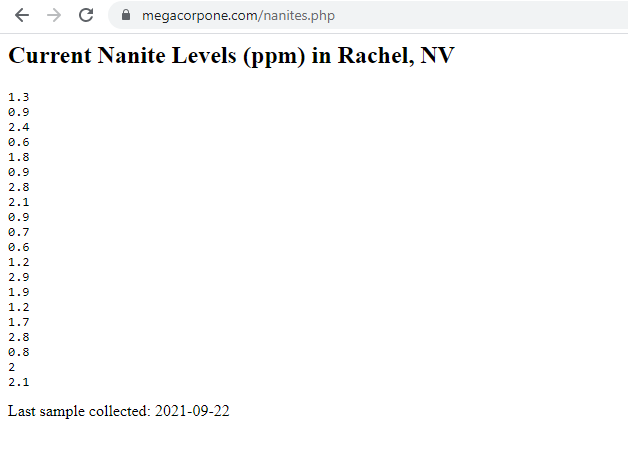
\includegraphics[width=0.55\textwidth]{images/lab1/nanite.PNG}
    \caption{./nanites.php}
    \label{fig:nanites.php}
\end{figure}

La sécurité du site WEB passe aussi par une bonne gestion des headers de celui-ci. Si nous observons les headers HTTP sur une page HTML quelconque, nous obtenons des informations sur le type et la version du serveur WEB (voir figure \ref{fig:versionapache}). Il s'agit d'une information utile pour diriger ses recherches d'éventuelles vulnérabilités.

\begin{figure}[H]
    \centering
    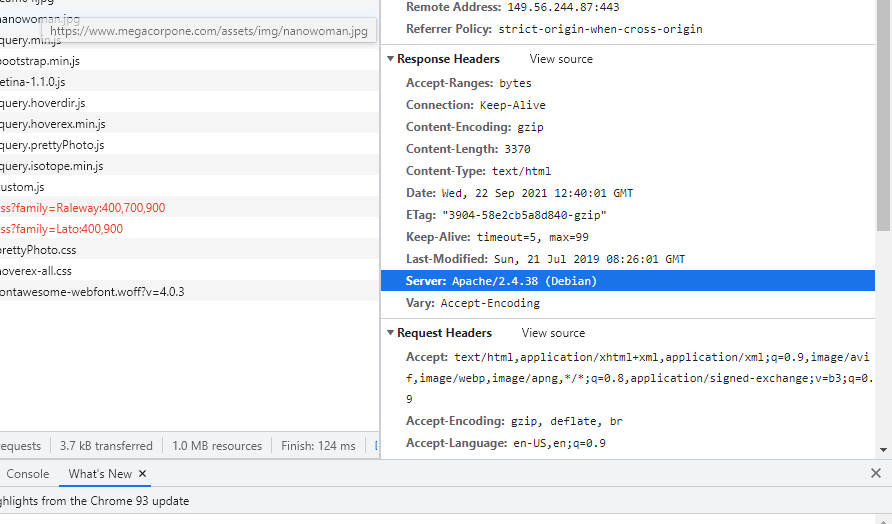
\includegraphics[width=0.90\textwidth]{images/lab1/version.PNG}
    \caption{Version Apache}
    \label{fig:versionapache}
\end{figure}

Nous pouvons également obtenir la version PHP grâce au header sur la page \textsc{nanites.php} (voir figure \ref{fig:versionphp}).

\begin{figure}[H]
    \centering
    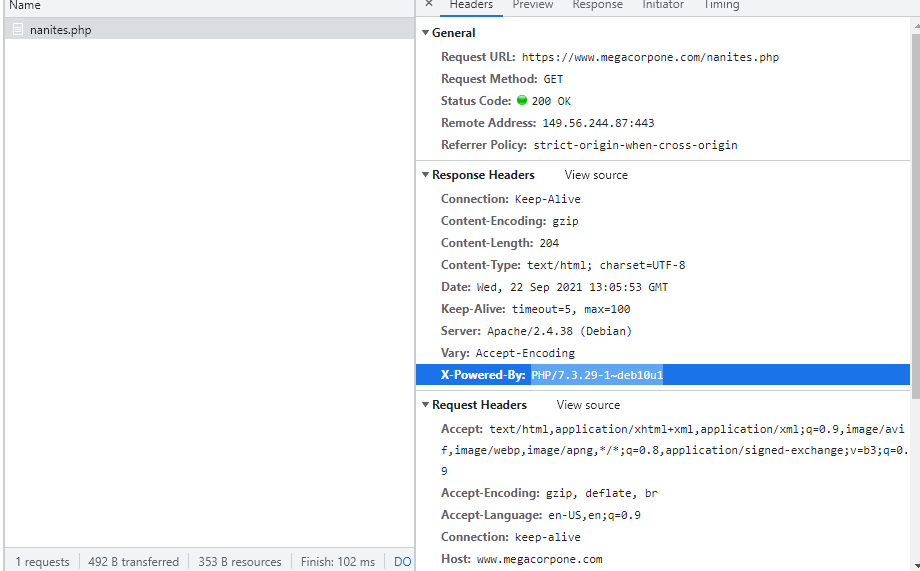
\includegraphics[width=0.90\textwidth]{images/lab1/versionphp.PNG}
    \caption{Version PHP}
    \label{fig:versionphp}
\end{figure}
 
Pour analyser d'autres potentielles vulnérabilités concernant les headers, nous allons sur \url{https://securityheaders.com}. Ce site va analyser les headers d'une page donnée et nous dire en quoi certains headers peuvent être manquants ou problématiques.\\
Dans notre cas, on peut voir que certains headers sont manquants tel que le CSP (Content-Security-Policy) qui lutte contre les attaques de type XSS (voir figure \ref{fig:missingheaders}).

\begin{figure}[H]
    \centering
    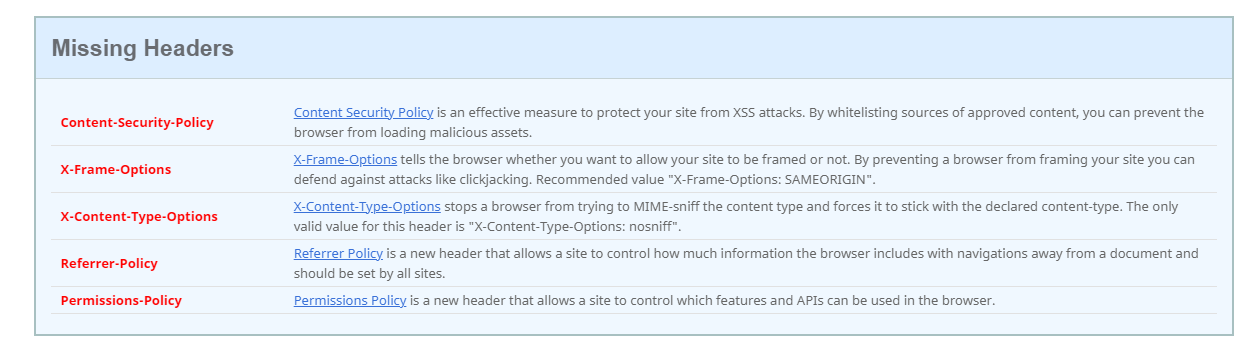
\includegraphics[width=0.90\textwidth]{images/lab1/missingheaders.PNG}
    \caption{Headers HTTP manquant}
    \label{fig:missingheaders}
\end{figure}

La page de contact nous permet d'accéder à plusieurs informations concernant des membres clés de l'entreprise (voir figure \ref{fig:contact}). En effet, ces informations peuvent être très utiles à des fins de phishing et de social engineering. 

\begin{figure}[H]
    \centering
    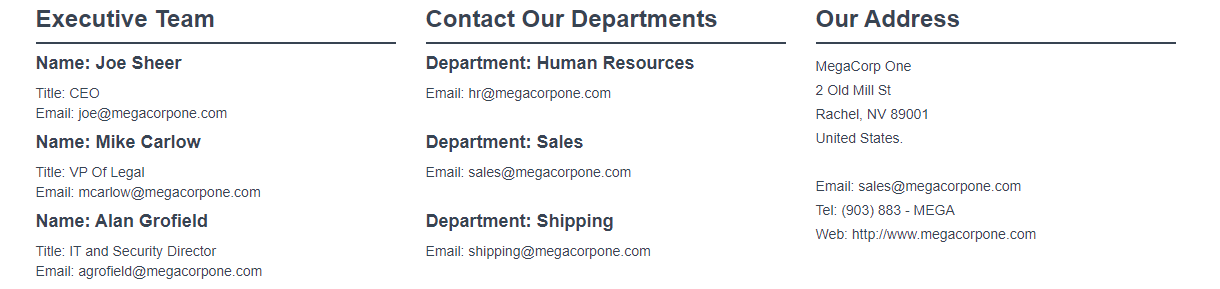
\includegraphics[width=0.85\textwidth]{images/lab1/Contact.PNG}
    \caption{Page de contact}
    \label{fig:contact}
\end{figure}

\subsection{Twitter}\label{sec:twitter}
Sous la rubrique \textsc{About} sur site, nous pouvons voir divers employés ainsi que leur Twitter.
Il s'agit d'une banque de données sans fin pour les hackers. Nous commençons donc par analyser le profil de chaque employé afin d'y trouver de potentielles informations. Nous y découvrons l'année de naissance de 2 personnes :
\begin{itemize}
    \item Joe Sheer (CEO) : 1968
    \item Tom Hudson (Lead Designer) : 1977
\end{itemize}
Cette information peut sembler banale, mais elle est bien souvent la clé d'un code pin ou d'un mot de passe.\\[0.2cm]

En faisant de plus amples recherches sur Twitter en cherchant \textsc{MegacorpOne}, nous tombons sur un selfie d'un certain William Adler qui dit être un nouvel employé (voir figure \ref{fig:selfie}). Nous pouvons apercevoir un post-it avec un identifiant et un mot de passe collé sur l'écran du poste de travail.
\begin{figure}[H]
    \centering
    
\includegraphics[width=0.65\textwidth]{images/lab1/twitter.jpg}
    \caption{Selfie compromettant sur twitter}
    \label{fig:selfie}
\end{figure}

\subsection{Informations sur le nom de domaine}
Voici les divers sous-domaines que https://searchdns.netcraft.com nous renvoie lorsque l'on cherche \emph{megacorpone.com} (voir figure \ref{fig:subdomain}).

\begin{figure}[H]
    \centering
    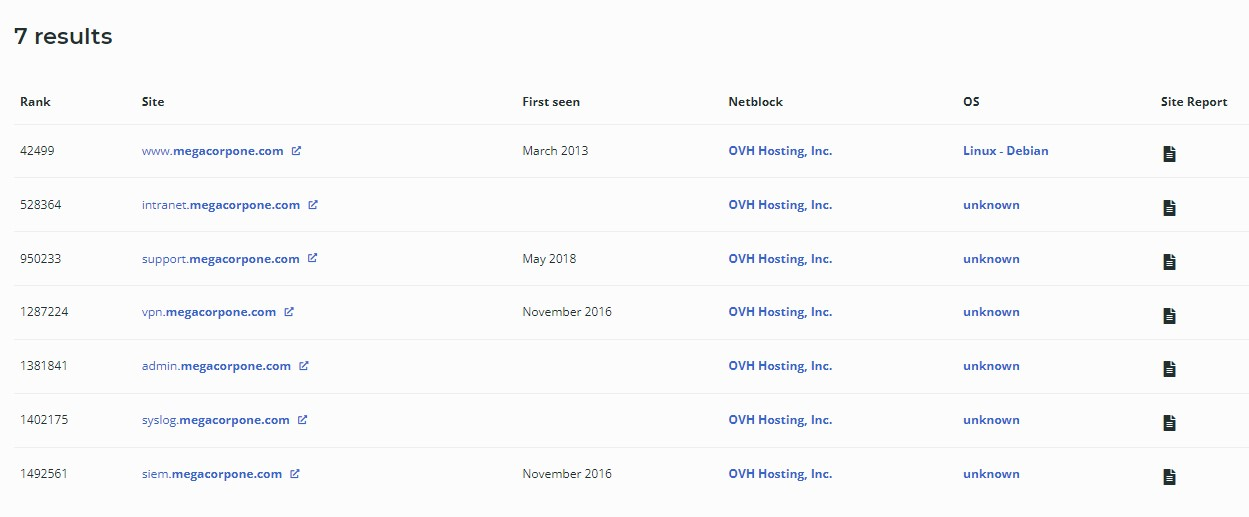
\includegraphics[width=0.80\textwidth]{images/lab1/subdomain.jpg}
    \caption{Les différents sous-domaines trouvés par netcraft}
    \label{fig:subdomain}
\end{figure}

\subsection{Informations complémentaires sur le site Web}
Grâce au certificat et à l'IP, nous pouvons obtenir d'autres informations telles que la localisation de l'IP, l'adresse de l'entreprise ou encore la date de création du site internet.
\begin{figure}[H]
    \centering
    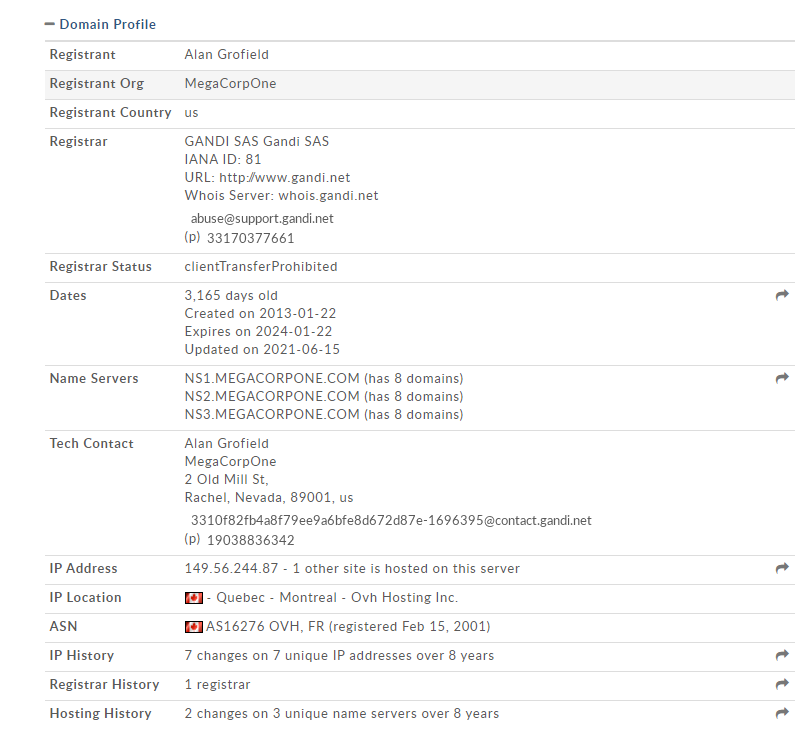
\includegraphics[width=0.75\textwidth]{images/lab1/certificat.png}
    \caption{Certificat et IP}
    \label{fig:certificat}
\end{figure}

Ensuite, à l'aide du moteur de recherche Shodan (https://www.shodan.io), nous pouvons obtenir davantage d'informations sur le site web de \textbf{Megacorpone} telles que les technologies web utilisées, certains ports ouverts, les versions des applications web et la version de l'OS, ainsi que certaines vulnérabilités associées aux versions trouvées des applications web. 
\begin{figure}[H]
    \centering
    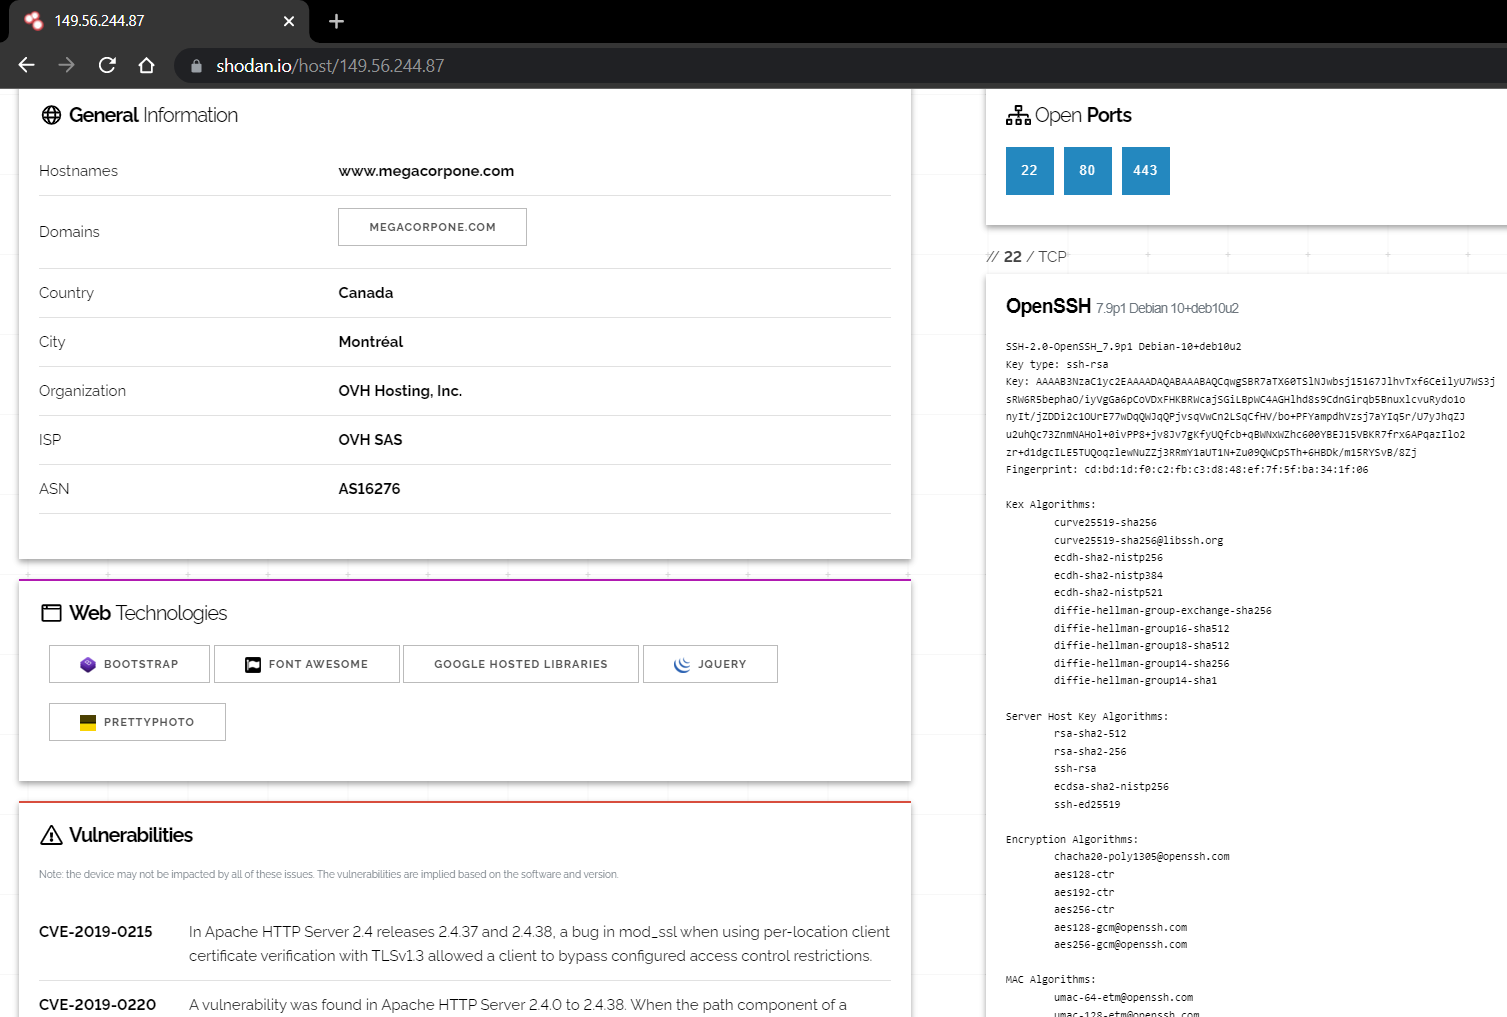
\includegraphics[width=0.75\textwidth]{images/lab1/shodan.png}
    \caption{Résultats Shodan}
    \label{fig:shodan}
\end{figure}





















\newpage
\section{Scanning et énumération} \label{sec:scanning}
Pour une meilleure lecture des résultats obtenus, nous utilisons la base de données de metasploit afin de stocker les résultats de nos divers scans. Nous commençons donc par créer celle-ci grâce à la commande \emph{msfdb init}.

\subsection{Découverte des hôtes}
Une première étape est de lister tous les hôtes et tous les sous-réseaux. Pour cela, nous commençons par faire un scan classique (sans options) et un scan ARP (voir annexe \ref{app:ARP}) sur 10.180.0.0/16. De cette manière, nous découvrons 3 sous-réseaux avec un total de 10 machines. Ensuite, nous retentons de scanner chacune des adresses IP avec \textbf{-O} pour tenter de découvrir l'OS de ces machines. Une fois cela fait, nous obtenons une base de données pleine d'informations utiles (voir figure \ref{fig:hosts}).

\begin{figure}[H]
    \centering
    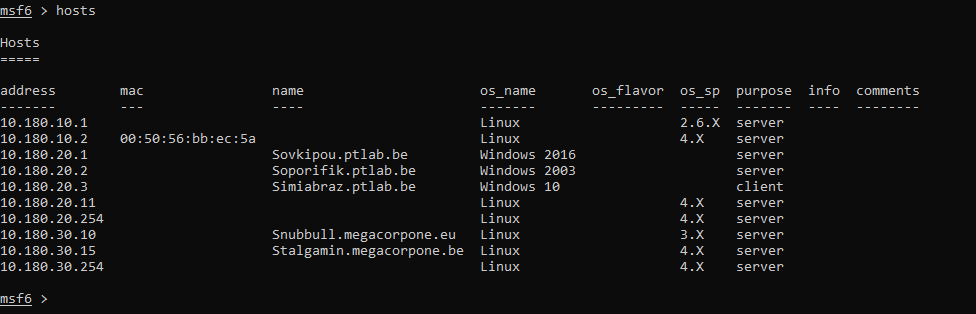
\includegraphics[width=0.90\textwidth]{images/lab2/hosts.png}
    \caption{Découverte des hôtes}
    \label{fig:hosts}
\end{figure}

\subsection{Découverte des services}
Nous allons maintenant pouvoir commencer à scanner chacune des machines afin d'en savoir plus sur les services disponibles. Voici les divers scans que nous avons effectués pour chacun des hôtes :
\begin{enumerate}
    \item \textsc{db\_nmap  -sV -sT -p- <IP>}
    \item \textsc{db\_nmap  -sV -sS -p- <IP>}
    \item \textsc{db\_nmap  -sV -sX -p- <IP>}
    \item \textsc{db\_nmap  -sV -sU <IP>}
\end{enumerate}
Pour plus d'informations sur les diverses options utilisées, voir l'annexe \ref{app:nmap}.\\

Après les divers scans, nous observons la base de données metasploit (\textbf{voir annexe \ref{app:services}}). 

\subsection{Smb-Os-Discovery}
Nous pouvons observer que nous avons un service \textsc{NetBios} sur la machine \textsc{Sovkipou.ptlab.be}. Nous pouvons vérifier son OS grâce à un script proposé par nmap : smb-os-discovery (voir figure \ref{fig:smb-os-discovery}).
\begin{figure}[H]
    \centering
    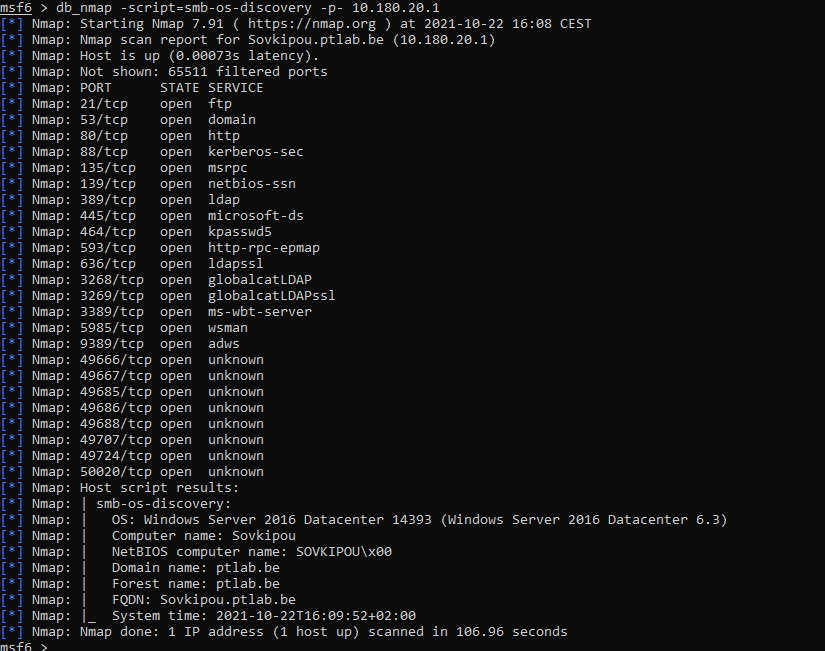
\includegraphics[width=0.80\textwidth]{images/lab2/smb.png}
    \caption{Smb-OS-Discovery}
    \label{fig:smb-os-discovery}
\end{figure}

\subsection{Découverte du SNMP}\label{sec:snmp}
Après avoir fait un scan UDP plus approfondi, nous avons découvert un service SNMP sur \textsc{Sovkipou.ptlab.be}. SNMP est très intéressant pour de potentiels attaquants. En effet, il permet de façon assez simple de faire des requêtes afin d'extraire des informations intéressantes. Dans notre cas, nous avons pu extraire divers username de l'Active Directory (voir figure \ref{fig:snmp}).
\begin{figure}[H]
    \centering
    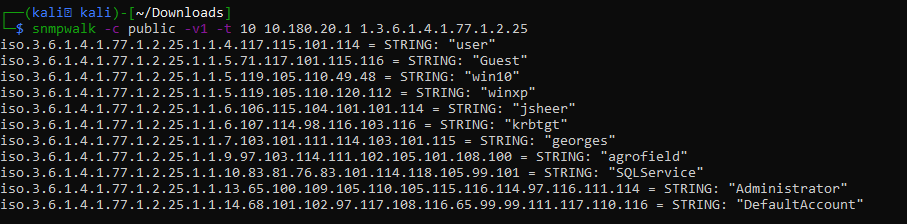
\includegraphics[width=0.90\textwidth]{images/lab2/snmpwalk.png}
    \caption{Extraction des usernames avec snmpwalk}
    \label{fig:snmp}
\end{figure}

\subsection{Découverte d'un appareil android}
Nous avions également trouvé un autre appareil avec l'adresse 10.180.20.11 lors de découverte du réseau. Étant donné que nous n'avons pas plus d'information à son sujet dans la base de données, nous décidons de recommencer un scan plus intensif. Nous découvrons alors qu'il s'agit d'un appareil android avec pour seul service disponible \emph{freeciv} (voir figure \ref{fig:android}).

\begin{figure}[H]
    \centering
    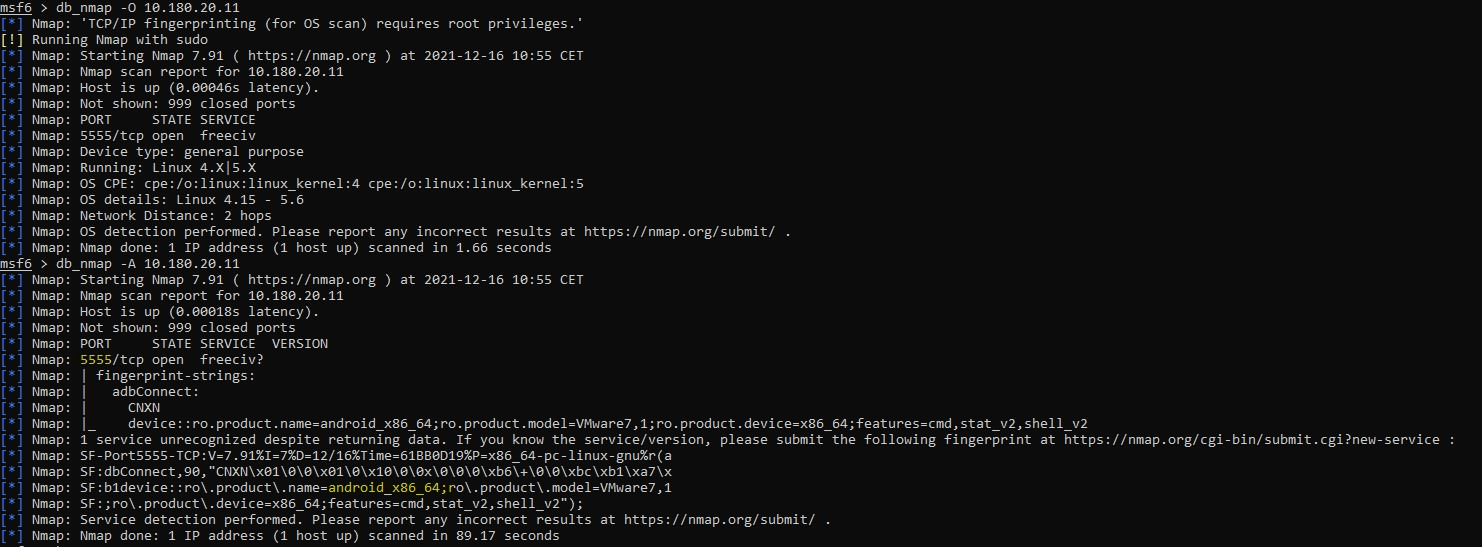
\includegraphics[width=1\textwidth]{images/lab2/android.jpg}
    \caption{Découverte d'un appareil android}
    \label{fig:android}
\end{figure}


























\newpage
\section{Recherche de vulnérabilités} \label{sec:vulnsearch}
Afin de connaître les différentes vulnérabilités, nous utilisons 2 outils différents :
\begin{itemize}
    \item Nmap (déjà utilisé précédemment)
    \item Nessus
\end{itemize}

\subsection{Analyse des vulnérabilités avec Nmap}
    Nmap propose une série de scripts de différents types. Il est également possible de réaliser un scan avec l'entièreté des scripts d'un type particulier. Dans notre cas, nous allons utiliser les scripts \textsc{vuln} afin d'analyser les services susceptibles d'être concernés par une CVE connue. A nouveau, grâce à la base de données de metasploit, nous pouvons réaliser les scans sur les différents hosts et obtenir un résultat résumé.\\ \\
    Nous lançons donc "\textsc{db\_nmap -sV --script vuln <IP>}" sur toutes les machines. Après cela, nous pouvons observer un nombre important de CVE, susceptibles d'être exploitées, signalé par nmap (voir figure \ref{fig:vulnsnmap}). Comme beaucoup de CVE signalées ne semblent pas correctes ou intéressantes à première vue, nous passons sur Nessus qui nous sera plus pratique afin de cibler les possibles points d'entrée sur le système.

\begin{figure}[H]
    \centering
    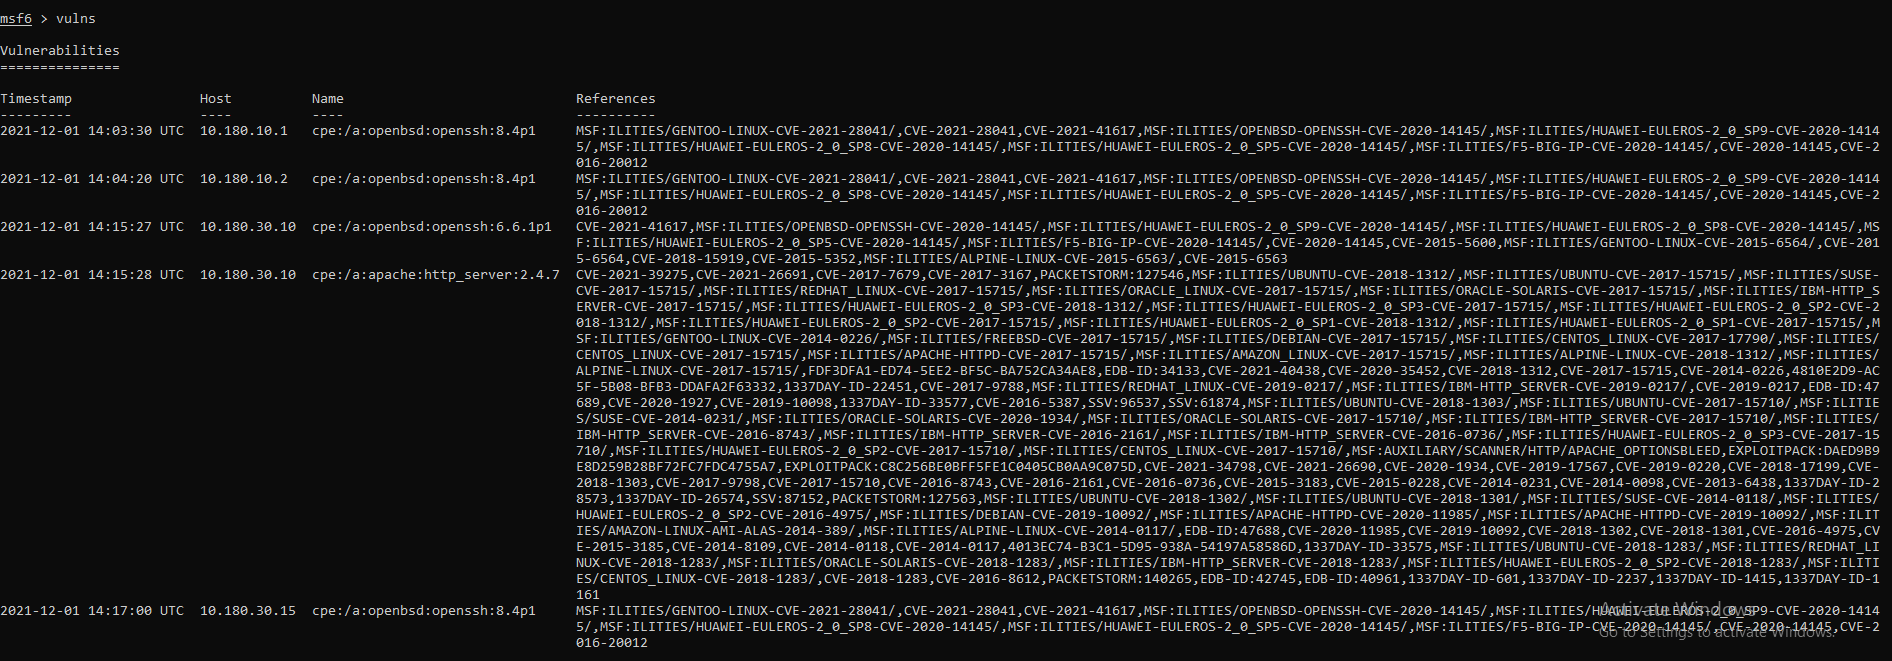
\includegraphics[width=1\textwidth]{images/lab3/resume.png}
    \caption{Collection des CVE - Nmap}
    \label{fig:vulnsnmap}
\end{figure}

\subsection{Analyse des vulnérabilités avec Nessus}
Grâce à Nessus, nous avons pu identifier certaines failles critiques ainsi qu'énumérer des éléments que nous n'avions pas découverts auparavant. Nous avons fait l'analyse sur les hôtes suivants :
\begin{itemize}
    \item 10.180.20.1 - \textsc{Sovkipou.ptlab.be}
    \item 10.180.20.2 - \textsc{Soporifik.ptlab.be}
    \item 10.180.20.3 - \textsc{Simiabraz.ptlab.be}
    \item 10.180.30.10 - \textsc{Snubbull.megacorpone.be}
    \item 10.180.30.15 - \textsc{Stalgamin.megacorpone.be}
\end{itemize}
Par la suite, nous avons fait un scan conçu pour les applications Web sur les 2 machines du sous-réseau 30.\\
Un rapport détaillé sur les vulnérabilités est disponible dans l'\textbf{annexe \ref{app:rapportvuln}}.




\newpage
\section{Exploitation et élévation de privilèges} \label{sec:exploitation}
\subsection{Wifi}\label{sec:wifi}

Afin d'avoir un point d'accès directement dans le réseau de l'entreprise, nous avons utilisé le point d'accès wifi \textsc{Ikki}. Grâce à l'outil \emph{wifite}, nous avons pu assez simplement retrouver le mot de passe de celui-ci (voir figure \ref{fig:wifi}). Cet outil fonctionne en 5 grandes étapes : 
\begin{enumerate}
    \item Découverte des SSID disponibles
    \item Écoute des requêtes sur le point d'accès
    \item Envoi de requêtes pour déconnecter des clients
    \item Interception de clé WPA2
    \item Tentative de déchiffrement grâce à une wordlist
\end{enumerate}

\begin{figure}[H]
    \centering
    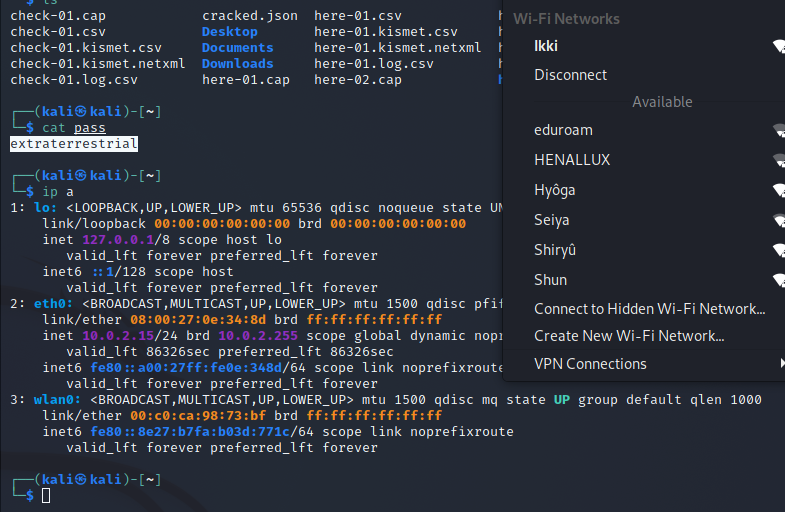
\includegraphics[width=0.8\textwidth]{images/lab4/WIFICRACKED.PNG}
    \caption{Découverte du mot de passe du point wifi "Ikki"}
    \label{fig:wifi}
\end{figure}




\subsection{Active Directory - Windows}\label{sec:wordlist}

Tout d'abord, nous avions réussi à avoir un accès sur le share SMB par "chance". En effet, nous avions pu découvrir les noms d'utilisateurs disponibles lors de l'énumération avec snmpwalk. Nous savions donc qu'il existait un username \emph{"user"}. Nous avons donc tenté de nous y connecter avec cet utilisateur et comme nous connaissions bien les personnes qui ont mis en place l'infrastructure, nous avons deviné que le mot de passe s'agissait de \emph{"Tigrou007"}. De cette manière, nous découvrons plusieurs sharename auxquels nous n'avons pas tous accès (voir figure \ref{fig:smbuser}).

\begin{figure}[H]
    \centering
    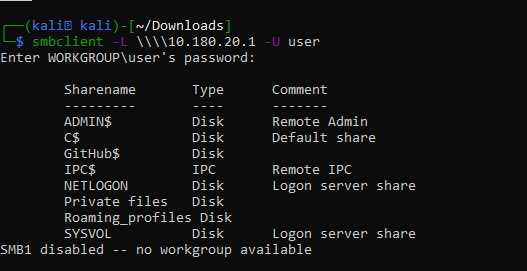
\includegraphics[width=0.4\textwidth]{images/lab4/smbuser.PNG}
    \caption{Découverte des différents share SMB grâce à "user"}
    \label{fig:smbuser}
\end{figure}

Dans l'un de ces partages, nous avons trouvé une wordlist comprenant tous les mots de passe leak de l'active directory. Un fichier qui ne devrait sans doute pas exister, d'autant plus dans un dossier partagé.

\subsubsection{Windows XP}
Nous créons un "user\_file" contenant tous les usernames que l'on a pu trouver avec snmp. Puis nous tentons un premier brute force du service SMB avec ce user\_file ainsi qu'une wordlist de mot de passe. Nous trouvons ainsi le mot de passe d'un utilisateur : winxp (voir figure \ref{fig:firstbrute}).

\begin{figure}[H]
    \centering
    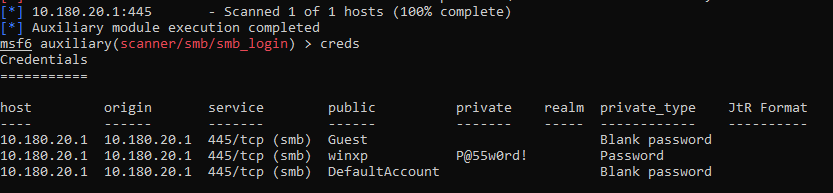
\includegraphics[width=1\textwidth]{images/lab4/brute_smb.PNG}
    \caption{Brute force SMB - WinxP}
    \label{fig:firstbrute}
\end{figure}

Maintenant que nous avons une nouvelle paire d'identifiant, nous tentons de procéder à un exploit qui se base sur la vulnérabilité \textsc{EternalBlue} que nous avons découverte lors de la recherche de failles (ms17\_010). Après avoir essayé divers exploit sur le contrôleur de domaine, nous comprenons que ces identifiants ne nous serviront pas pour cette machine. Nous essayons donc à nouveau sur la Windows XP et nous réussissons à mettre en place une backdoor (voir figure \ref{fig:meterpreter}).

\begin{figure}[H]
    \centering
    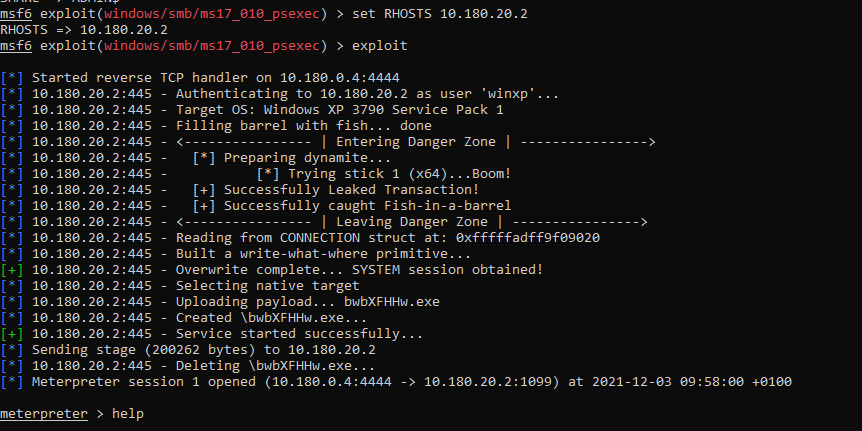
\includegraphics[width=1\textwidth]{images/lab4/meterpreter.PNG}
    \caption{Déploiement d'une backdoor sur \textsc{Soporifik.Ptlab.be}}
    \label{fig:meterpreter}
\end{figure}

Après cela, nous avons mis en place un accès RDP pour accéder à la machine avec plus de facilité.\\ (Voir figure \ref{fig:getgui} et \ref{fig:winxp})

\begin{figure}[H]
    \centering
    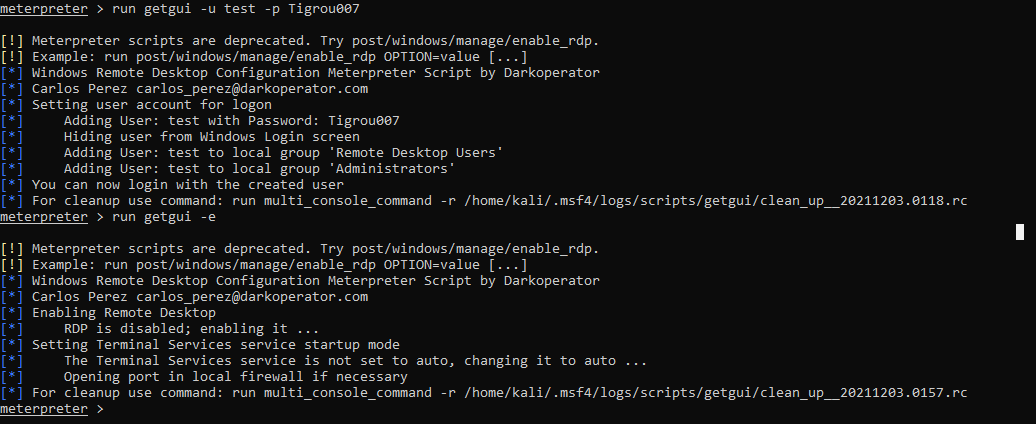
\includegraphics[width=1\textwidth]{images/lab4/rdp.PNG}
    \caption{Mise en place d'un accès RDP sur \textsc{Soporifik.Ptlab.be}}
    \label{fig:getgui}
\end{figure}

\begin{figure}[H]
    \centering
    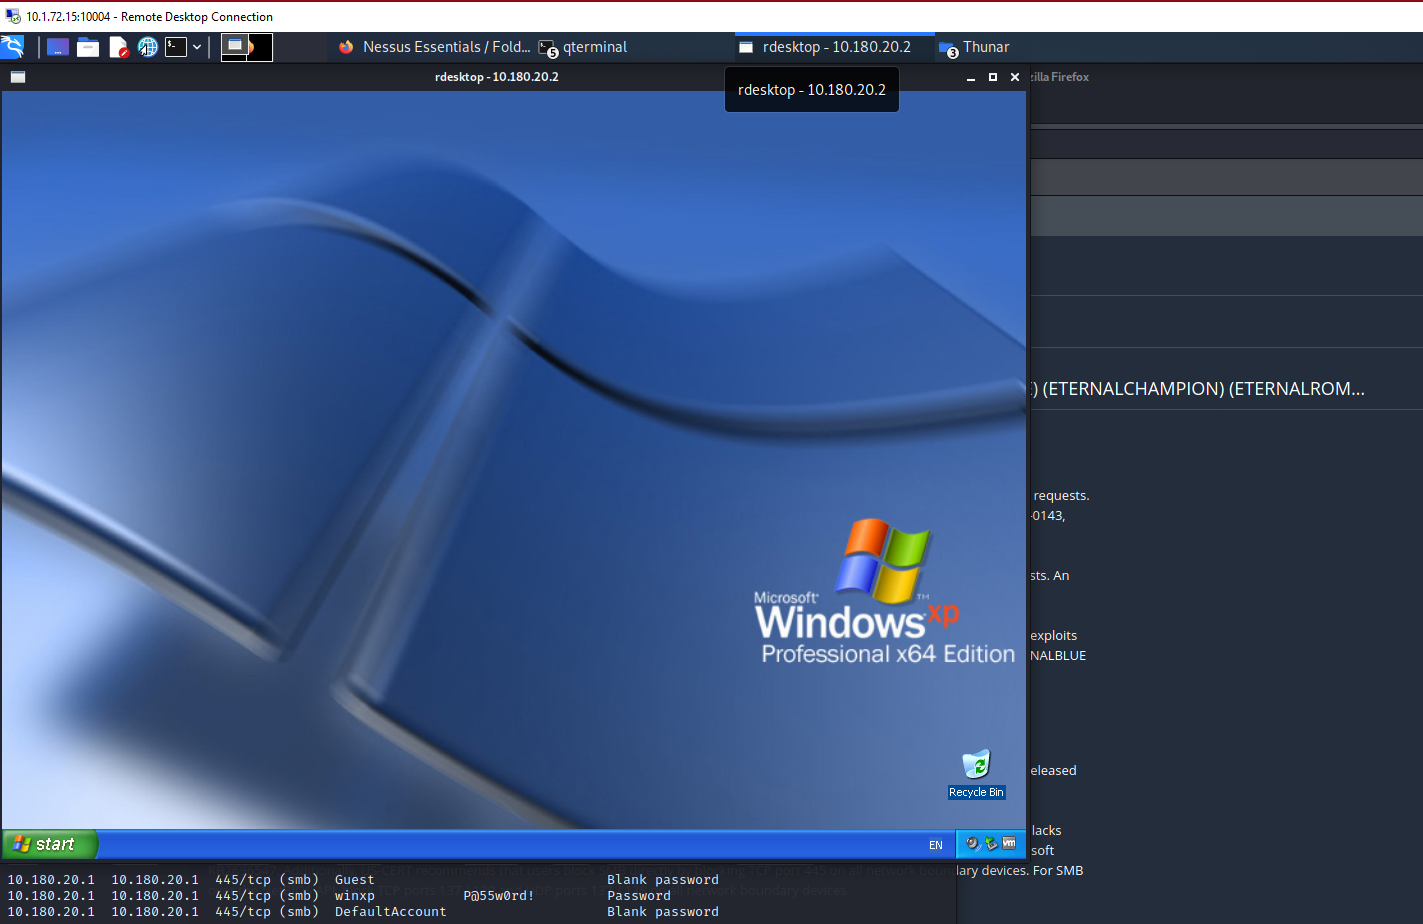
\includegraphics[width=1\textwidth]{images/lab4/winxp_access.png}
    \caption{Accès à la machine Windows XP}
    \label{fig:winxp}
\end{figure}

Nous avons réussi à obtenir un accès, mais malheureusement il ne nous est pas suffisant pour accéder au contrôleur de domaine. Nous décidons alors de déterminer quel identifiant est l'administrateur de l'Active Directory. Pour cela, nous nous servons également de la vulnérabilité MS17\_010 (voir figure \ref{fig:enumadmin}).

\begin{figure}[H]
    \centering
    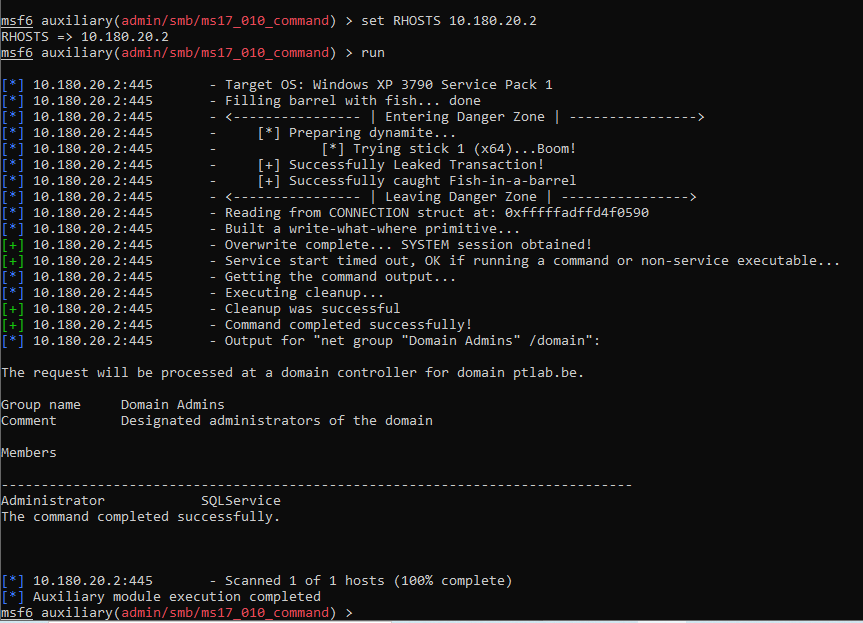
\includegraphics[width=0.8\textwidth]{images/lab4/MS17_010.PNG}
    \caption{Énumération du compte administrateur}
    \label{fig:enumadmin}
\end{figure}

Après nous être rappelé avoir découvert une wordlist avec des mots de passe leak sur le SMB, nous décidons de retenter un brute force sur l'identifiant unique "SQLService" avec cette wordlist. Nous obtenons ainsi une nouvelle paire d'identifiants (voir figure \ref{fig:secondbrute}).

\begin{figure}[H]
    \centering
    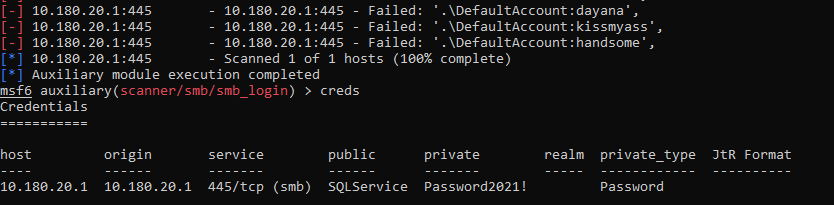
\includegraphics[width=0.8\textwidth]{images/lab4/secondbruteforce.PNG}
    \caption{Second brute force - SqlService}
    \label{fig:secondbrute}
\end{figure}

\subsubsection{Windows 10}

Nous tentons donc de nous connecter en RDP sur la windows server, mais la connexion est refusée par faute de certificat, nous tentons de même sur la WindowsXP mais nous obtenons la même erreur. Nous tentons donc de nous connecter tout d'abord sur la 3ème machine, \textsc{Simiabraz.ptlab.be} (une Windows 10). (Voir figure \ref{fig:rdptowin}).

\begin{figure}[H]
    \centering
    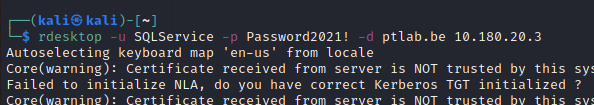
\includegraphics[width=0.8\textwidth]{images/lab4/rdptowin.PNG}
    \caption{Connexion RDP à la Windows 10 (\textsc{Simiabraz.ptlab.be})}
    \label{fig:rdptowin}
\end{figure}

Nous obtenons bien un accès RDP sur cette machine.

\subsubsection{Windows Server}
Nous tentons maintenant une connexion RDP sur \textsc{Sovkipou.ptlab.be} depuis la Windows 10. Cette fois-ci, plus de soucis avec les certificats. Nous obtenons bel et bien un accès sur le contrôleur de domaine, et ce, en administrateur (voir figure \ref{fig:admintoserv}).


\begin{figure}[H]
    \centering
    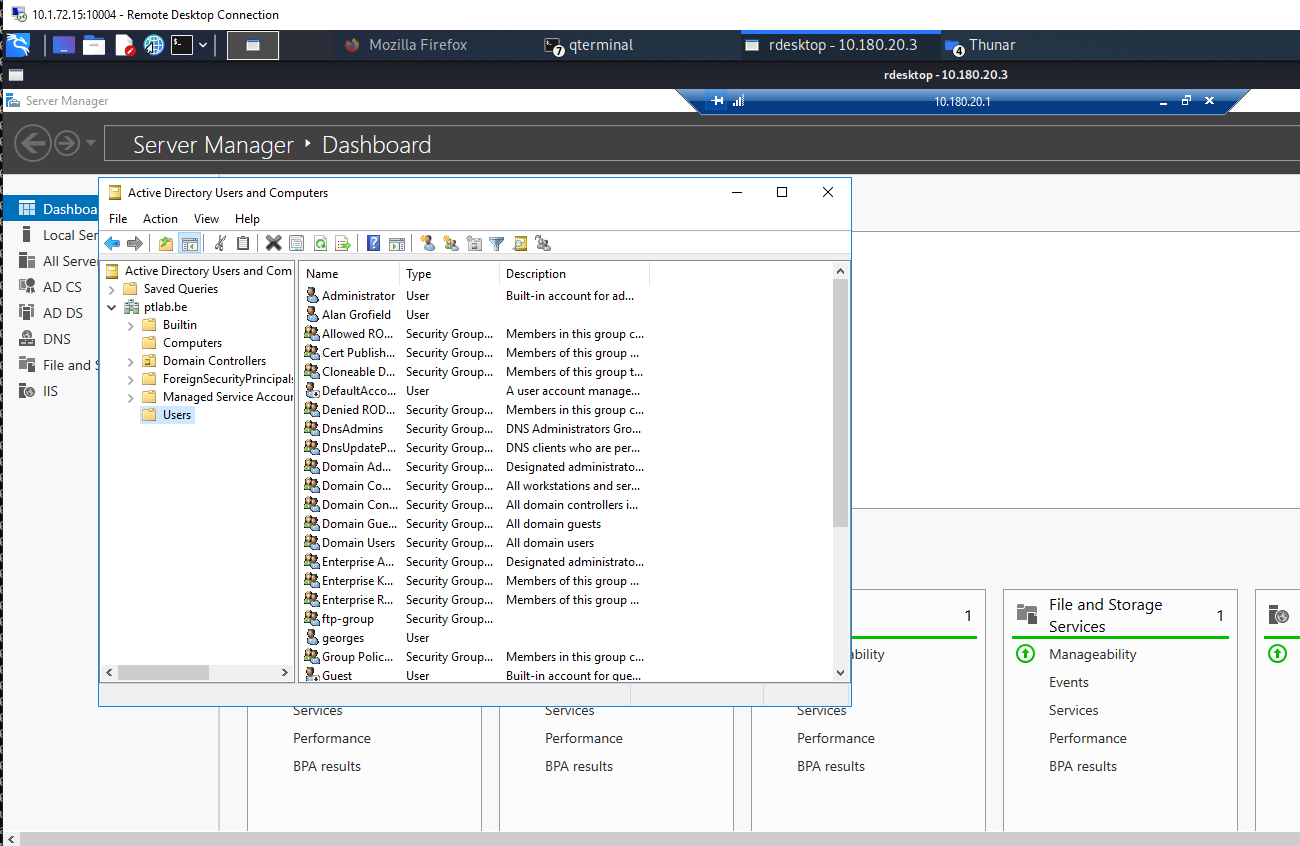
\includegraphics[width=0.8\textwidth]{images/lab4/admintoserv.PNG}
    \caption{Connexion RDP en administrateur sur la windows server}
    \label{fig:admintoserv}
\end{figure}









\subsection{Linux}\label{sec:linuxmdp}

Grâce aux scans de type web via le logiciel Nessus, nous avons eu la liste de tous les répertoires wordpress sur la machine Snubbull. (Voir annexe \ref{app:vulns5})\\
Cela nous a permis d'atteindre la page de connexion de Wordpress pour la gestion du site. De plus, étant donné que le site Wordpress était vulnérable à l'énumération des utilisateurs, les combinaisons de user/password étaient réduites. Dès lors nous avons tenté de deviner le mot de passe des deux utilisateurs référencés. Après quelques tentatives, nous avons retrouvé le mot de passe de l'utilisateur 'blogger' qui n'était d'autre que \emph{blogger}. Cela arrive encore fréquemment que le mot de passe soit le même que le nom d'utilisateur.\\\\
Dès lors, après avoir obtenu un accès à l'administration du site web wordpress, nous avons exploré les diverses fonctionnalités de Wordpress. Nous avons cherché un moyen d'upload un 'reverse\_shell' en PHP afin d'obtenir un terminal sur la machine cible. En explorant les rubriques de Wordpress, nous nous sommes rendus dans la section 'Slideshow' et nous avons remarqué différentes 'Slides' qui correspondaient aux noms des employés de Megacorpone. Ces 'Slides' faisaient référence aux différentes photos des employés se trouvant sur la page 'About-us' du site de Megacorpone.\\

\begin{figure}[H]
    \centering
    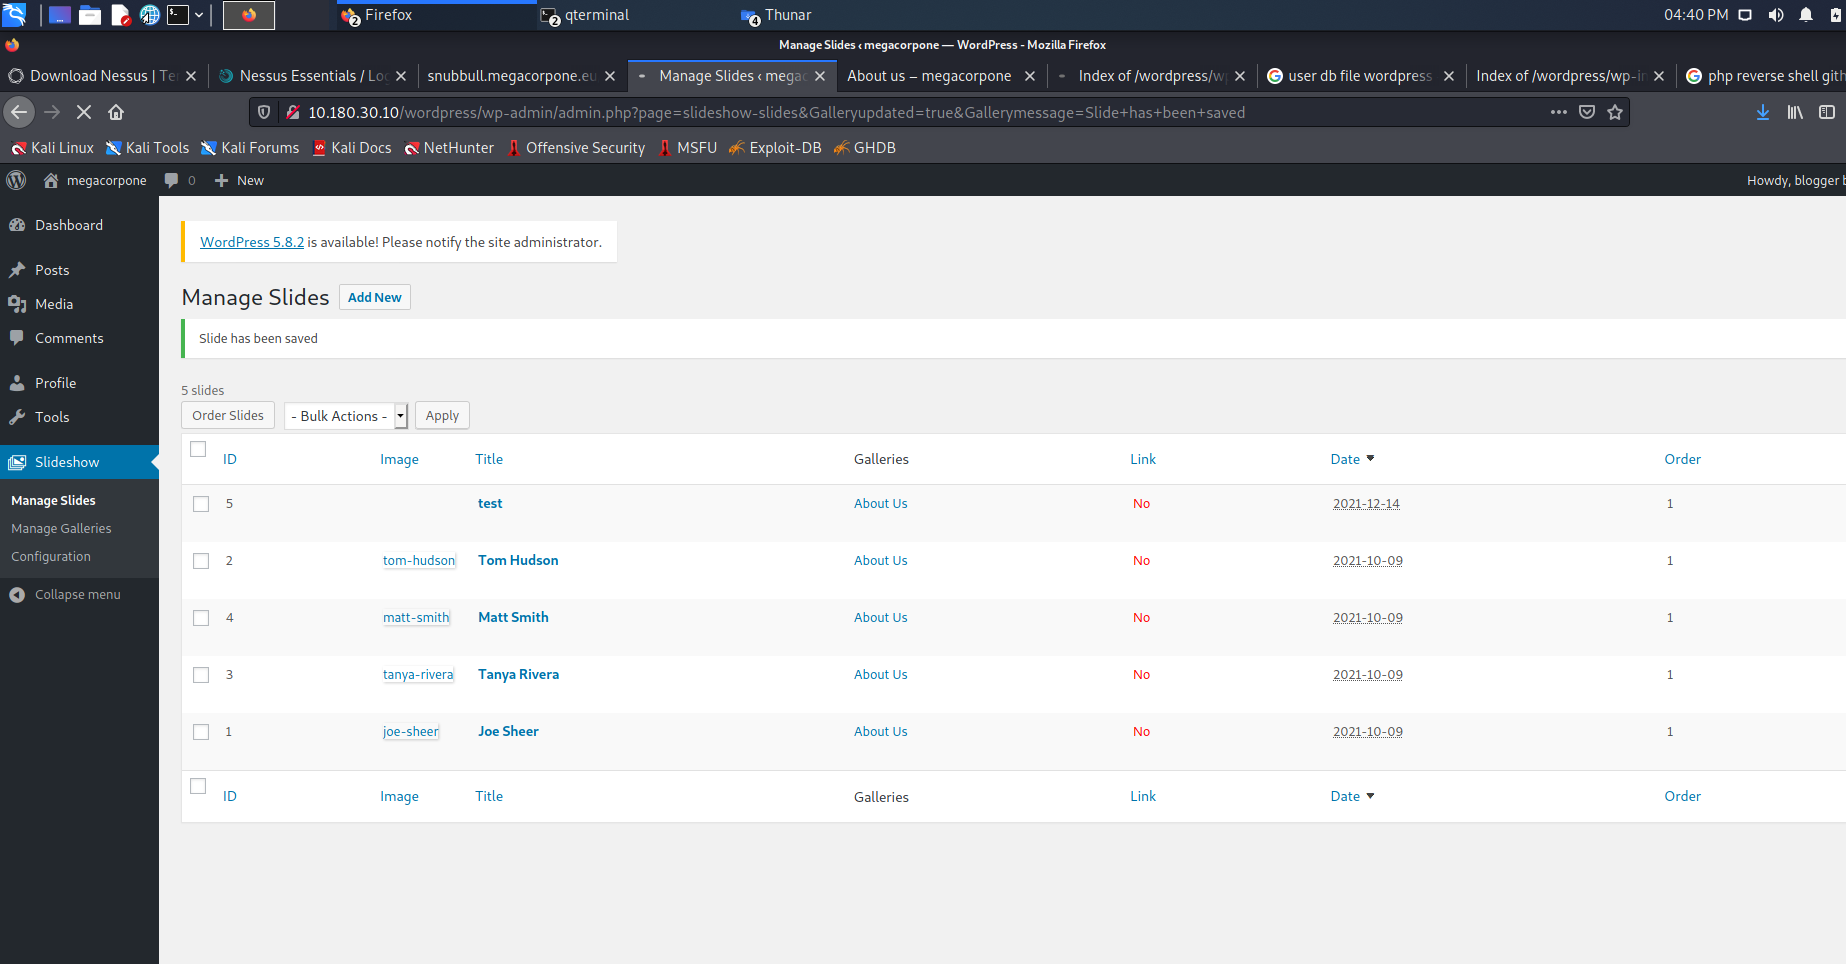
\includegraphics[width=0.8\textwidth]{images/lab4/wordpress_upload.png}
    \caption{Accès admin à la gestion du site Wordpress}
    \label{fig:wordpress}
\end{figure}

Nous avons donc tenté d'upload un 'reverse\_shell' en PHP dans la rubrique 'Slideshow' et ensuite naviguer dans le répertoire des uploads du site, afin d'y retrouver notre fichier uploadé. Nous n'étions pas sûrs que cela allait fonctionner, car il était indiqué que seuls des fichiers ayant comme format PNG, GIF, ou JPEG pouvaient être uploadés. Cependant, comme nous avions un accès administrateur à la gestion du site, l'upload de notre fichier en PHP a bien fonctionné. \cite{7}\\

Nous avons donc ouvert un terminal sur notre machine hôte afin d'écouter une connexion TCP entrante sur le port 1234 et sur l'IP du site (10.180.30.10). De ce fait, une fois que nous naviguions dans les fichiers uploadés et que nous accédions à notre fichier en PHP, cela nous a permis d'obtenir un accès terminal sur la machine cible.\\

\begin{figure}[H]
    \centering
    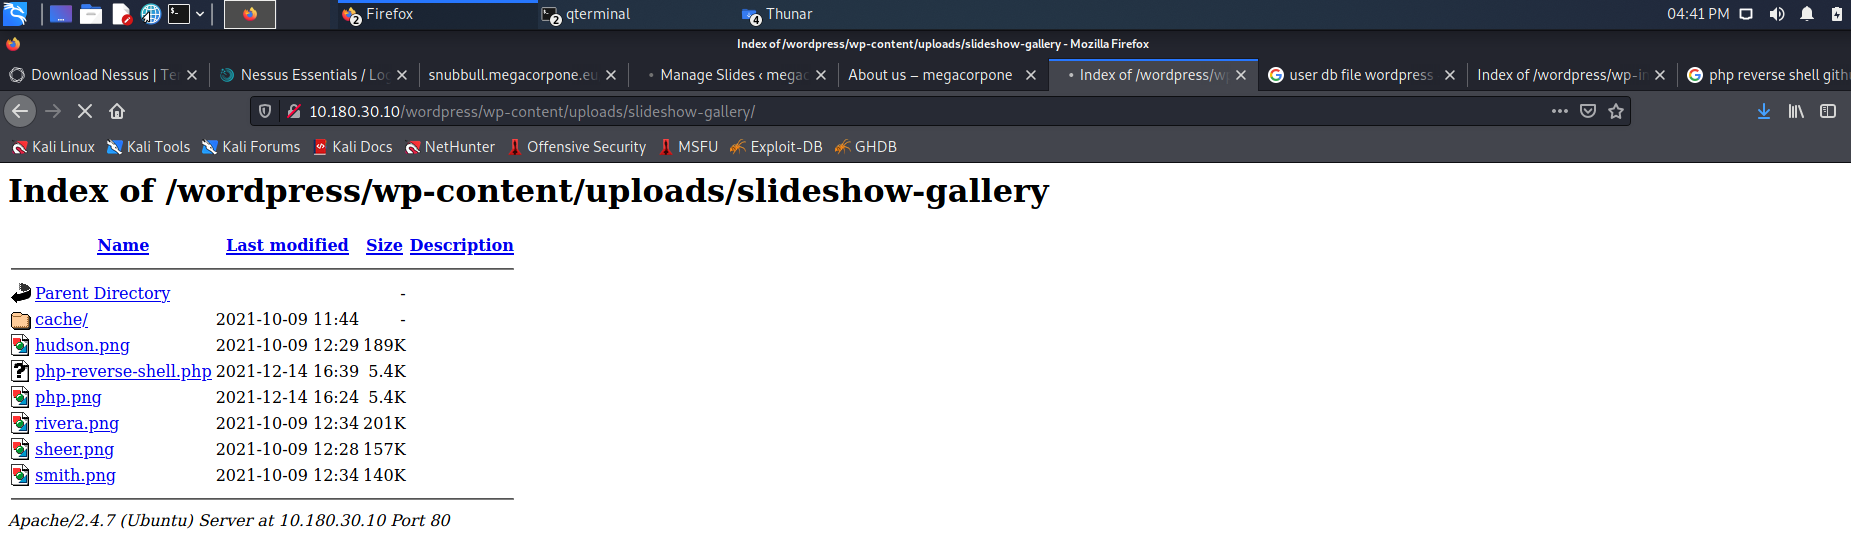
\includegraphics[width=0.8\textwidth]{images/lab4/reverse_shell.png}
    \caption{Upload de notre reverse\_shell en PHP}
    \label{fig:phpshell}
\end{figure}

Cependant, nous étions connectés en tant qu'utilisateur 'www-data'. La première chose à faire a été d'ouvrir un tty-shell car il ne nous est pas possible d'utiliser certaines commandes telles que le \emph{su} ou \emph{sudo} dans un reverse shell. Pour cela, nous utilisons python pour nous créer notre nouveau tty-shell \cite{6}: \textsc{python -c 'import pty; pty.spawn("/bin/sh")'}. \\\\ Ensuite, seule la commande 'strace' pouvait être lancée en mode \emph{sudo} sans devoir renseigner le mot de passe. Nous l'avons découvert en entrant la commande 'sudo -l' qui nous permet de retrouver les commandes qui peuvent être utilisées en sudo avec l'utilisateur actuel. Nous avons donc cherché un moyen d'élever nos privilèges à l'aide de la commande 'strace' et nos recherches ont été fructueuses, car un exploit avait déjà été réalisé pour cette version de sudo, et donc via une simple commande, nous sommes passés de 'www-data' à 'root'. Cette élévation de privilèges a été possible car la version de 'sudo' (1.8.9p5) était vulnérable à des failles de type élévation de privilèges ainsi qu'à une mauvaise configuration.\cite{4}

\begin{figure}[H]
    \centering
    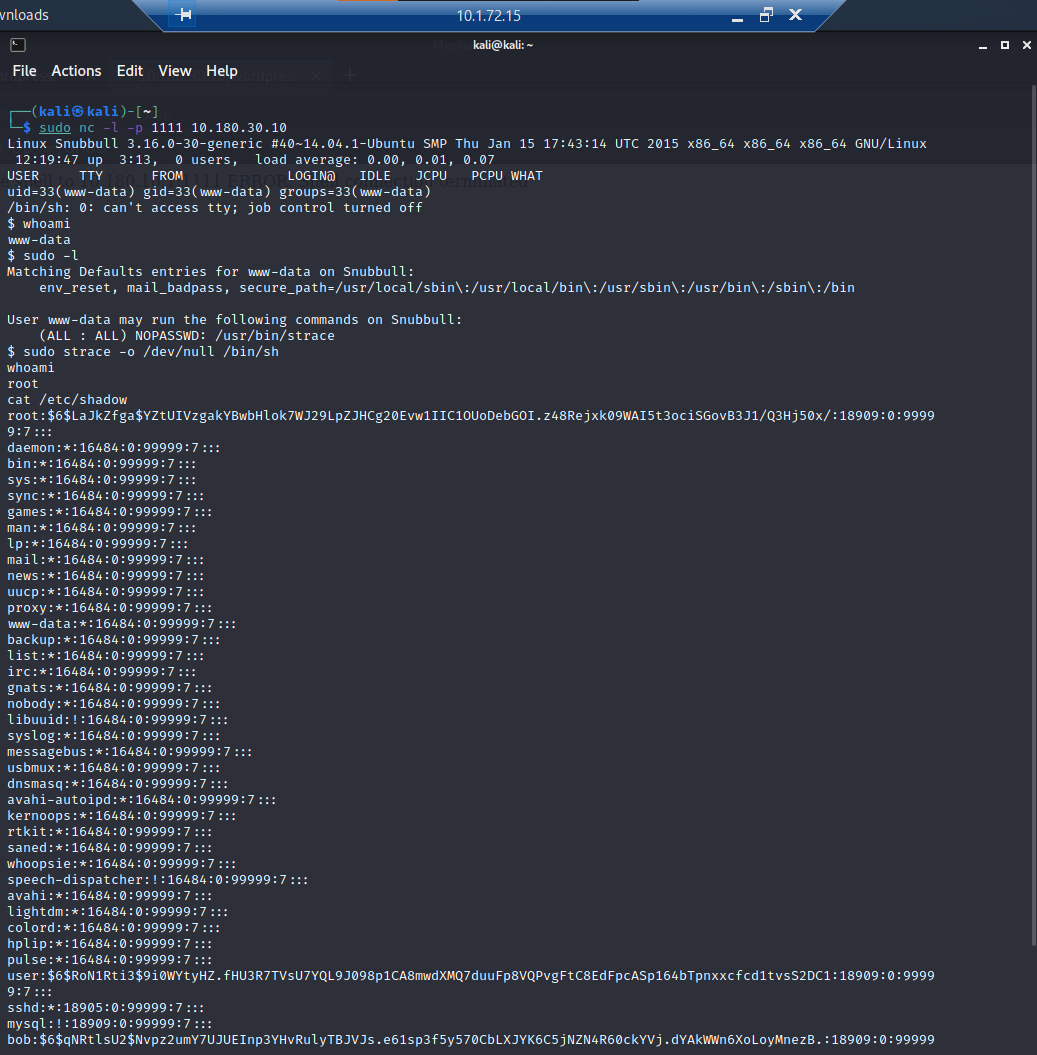
\includegraphics[width=0.8\textwidth]{images/lab4/shell_root_access_snubull.png}
    \caption{Élévation de privilèges depuis notre reverse\_shell}
    \label{fig:linuxprivesc}
\end{figure}

\newpage
\subsection{Android}

Lors de la phase d'énumération, nous avons remarqué la présence d'une machine Android ainsi que du service Freeciv qui est sur le port 5555.\\
En nous renseignant un peu sur ce service, nous avons retrouvé quelques CVE faisant références aux versions obsolètes de Freeciv. Dès lors, en cherchant comment nous allions pouvoir exploiter une éventuelle vulnérabilité, nous avons découvert le package 'adb' qui signifie \textbf{Android Debug Bridge} et qui est donc un outil en ligne de commande permettant de communiquer avec un appareil Android. Cet outil nous a donc permis de nous connecter à la machine Android, pour ensuite y obtenir un terminal. Une fois connecté à la machine, nous avons remarqué que nous étions connectés en tant que user 'shell' et donc nous avons recherché un moyen d'élever nos privilèges. De ce fait, la simple commande '\emph{su}' nous permet d'obtenir un accès root à la machine Android. \cite{8}

\begin{figure}[H]
    \centering
    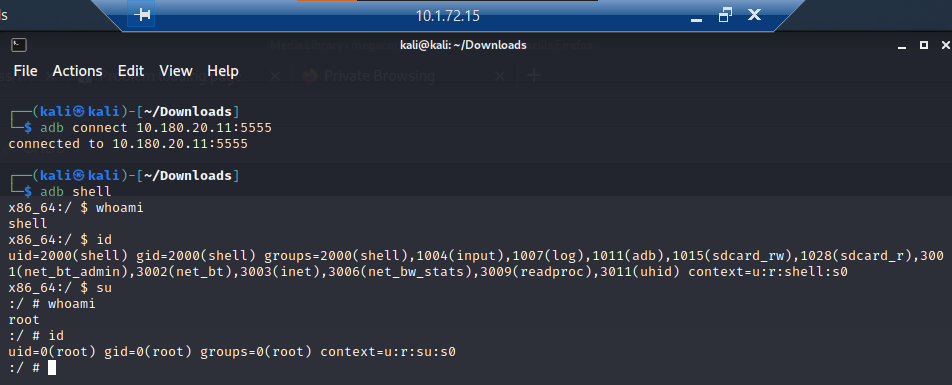
\includegraphics[width=0.8\textwidth]{images/lab4/android_shell.png}
    \caption{Accès à un shell 'root' sur la machine Android}
    \label{fig:androidshell}
\end{figure}


\newpage
\section{Résultats}

Cet audit de sécurité s'est avéré productif. En effet, nous avons pu déterminer de grands points de faiblesse sur le système d'information, tous étant énumérés lors de ce rapport. Dans l'état actuel du système d'information, nous avons réussi à compromettre 5 machines :
\begin{itemize}
    \item \textsc{Sovkipou.ptlab.be} (Windows Server) :\\
    Nous avons réussi à trouver les identifiants administrateur et nous avons également réussi à nous y connecter en RDP.
    \item \textsc{Soporifik.ptlab.be} (Windows XP) :\\
    Nous avons pu déterminer les identifiants locaux et grâce à une backdoor meterpreter, nous nous sommes créé un accès RDP.
    \item \textsc{Simiabraz.ptlab.be} (Windows 10) :\\
    Cette machine nous a surtout servi de pont vers la Windows Server. Elle nous fut très utile pour nous connecter en RDP à \textsc{Sovkipou.ptlab.be}.
    \item 10.180.20.11 : \\
    Cet appareil android était assez simple à compromettre et l'accès administrateur était presque direct.
    \item \textsc{Stalgamin.megacorpone.be} (Ubuntu) :\\
    Grâce à diverses vulnérabilités Wordpress, à la faiblesse du mot de passe "blogger" et grâce à la misconfiguration de sudo; nous avons pu obtenir un accès root au serveur Ubuntu.\\\\
\end{itemize}

En plus de tout cela, il nous a également été possible de nous connecter à l'infrastructure via le Wifi qui fut simple à craquer grâce à l'outil \emph{Wifite}.


















\newpage
\section{Conclusion}
En conclusion, les résultats obtenus lors de ce test de pénétration sur l'infrastructure de la société \textbf{Megacorpone} se sont avérés être très pertinents. En effet, nous avons constaté un manque considérable au niveau de la sécurité informatique de cette infrastructure. C'est-à-dire que des données sensibles de l'entreprise ont été trouvées, de nombreuses vulnérabilités en matière de sécurité ont été détectées et exploitées. Dès lors, nous avons établi certaines recommandations afin de corriger ces vulnérabilités, et de mieux sécuriser l'infrastructure en général.\\

Tout au long de ce test de pénétration, nous avons suivi la méthodologie \textbf{Kill Chain}. Cette méthodologie nous a été présentée en début d'année lors de l'introduction au cours de sécurité offensive. Cela nous a appris à respecter une chronologie bien précise, afin de réaliser au mieux ce test de pénétration.\\

Nous avons donc commencé par l'étape de reconnaissance qui nous a permis de recueillir des informations importantes sur l'infrastructure de la société, pour ensuite procéder à la phase d'énumération et de scanning, qui nous a permis de nous orienter de manière plus précise pour les étapes suivantes. Ces deux premières étapes constituent la base de tous tests d'intrusion. En effet, nous avons commencé la phase de recherche d'éventuelles vulnérabilités sur base des résultats obtenus lors des étapes précédentes, pour ensuite procéder à l'exploitation de ces vulnérabilités ainsi qu'à de potentielles élévations de privilèges.\\

Nous avons donc conclu que les mesures de sécurité mises en place au niveau de l'infrastructure de la société étaient insuffisantes lors de la réalisation de ce test, il est donc fortement recommandé d'appliquer certaines solutions présentées dans la section \nameref{sec:solutions}.




































\newpage \appendix
\section{Web}
\subsection{Robots.txt} \cite{1} \label{app:robots}
Robots.txt est un fichier texte que les webmasters créent pour indiquer aux robots Web (généralement les robots des moteurs de recherche) comment explorer les pages de leur site Web. Le fichier robots.txt fait partie du protocole d'exclusion des robots (REP), un groupe de normes Web qui régulent la façon dont les robots explorent le Web, accèdent et indexent le contenu, et diffusent ce contenu aux utilisateurs. Le REP comprend également des directives telles que des méta robots, ainsi que des instructions à l'échelle de la page, du sous-répertoire ou du site sur la façon dont les moteurs de recherche doivent traiter les liens (telles que « suivre » ou « nofollow »).

En pratique, les fichiers robots.txt indiquent si certains agents utilisateurs (logiciels d'exploration Web) peuvent ou non explorer des parties d'un site Web. Ces instructions d'exploration sont spécifiées en « interdisant » ou « autorisant » le comportement de certains (ou de tous) agents utilisateurs.

\section{Nmap}\label{app:nmap}

\subsection{Scan ARP}\label{app:ARP}
L'option \textbf{-P*} permet d'associer une option à la découverte des hosts lors du scan. De cette manière, l'option \textbf{-Pn} annulera les pings, ou encore \textbf{-PR} permettra une découverte ARP. D'autres options sur la découverte des hosts existent également. Les pings ARP sont très utiles car les hôtes peuvent bloquer assez facilement les pings classique ICMP mais ne bloquent généralement pas les requêtes ARP.

\subsection{Qu'est-ce que l'option \text{-sV} ?}
Il s'agit simplement d'une option permettant la détection de la version des différents services découverts. Pour plus d'information, consultez \url{https://nmap.org/book/vscan.html}.


\subsection{Différence entre \textsc{-sT} et \textsc{-sS}} \cite{2}
Pour bien comprendre, nous devons rappeler le TCP Handshake.
Lors d'une connexion TCP classique, le client envoie un flag \textsc{SYN}. Si le serveur possède son port fermé, il renverra \textsc{RST} (Reset) mais si le port est ouvert et que la connexion est autorisée, celui-ci renverra \textsc{SYN/ACK}. Le client devra alors renvoyer le flag \textsc{ACK} afin d'établir cette connexion.\\
-sT est une option permettant le scan TCP. Ce qui veut dire que l'on va utiliser le TCP handshake de manière classique sur chacun des ports que l'on veut tester.\\
-sS est une option permettant l'analyse \textsc{SYN}. Le TCP handshake va se faire de la même manière, si ce n'est que le client renverra un flag \textsc{RST} au lieu de \textsc{ACK} à la fin du handshake.\\\\
Les avantages à utiliser une analyse \textsc{SYN} : 
\begin{itemize}
    \item Permets de contourner des anciens IDS qui se basent sur un TCP handshake complet
    \item Les analyses ne sont généralement pas enregistrées par les applications
    \item Beaucoup plus rapide que des analyses TCP standards
\end{itemize}
Quels désavantages ?
\begin{itemize}
    \item Nécessite des privilèges root
    \item Les services instables sont parfois interrompus par les analyses SYN
\end{itemize}

\subsection{L'option \textsc{-p-}}
De base, nmap va scanner les 1000 ports les plus utilisés. L'option \textsc{-p} va permettre de sélectionner un range de port à analyser et \textsc{-p-} va permettre de sélectionner l'intégralité des ports pour l'analyse.

\newpage \section{Scan des différents services}\label{app:services}
\begin{figure}[H]
    \centering
    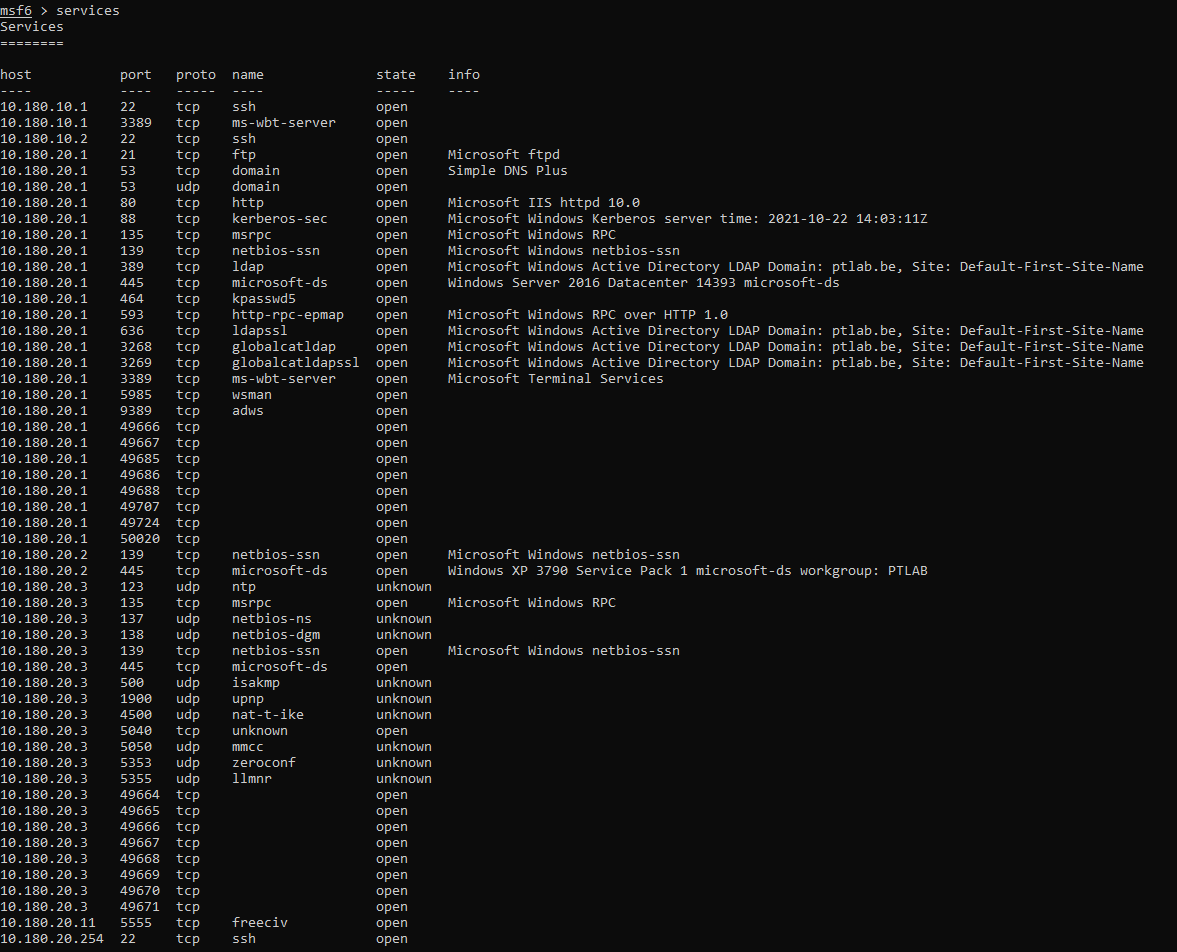
\includegraphics[width=1\textwidth]{images/lab2/services.png}
    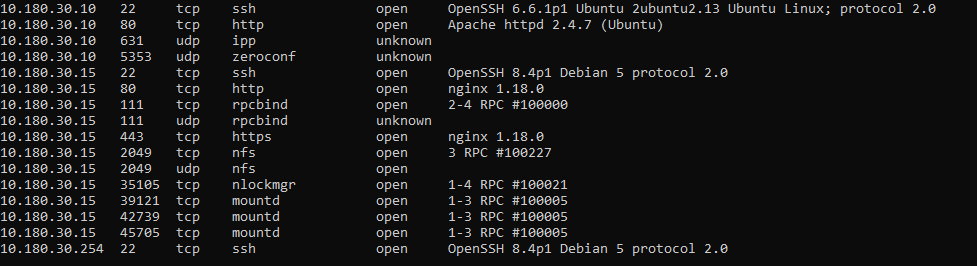
\includegraphics[width=1\textwidth]{images/lab2/hosts2.png}
    \caption{Découverte des services sur tous les hôtes}
    \label{fig:service}
\end{figure}

\newpage \section{Rapport de l'analyse des vulnérabilités}\label{app:rapportvuln}
\subsection{Basic Network Scan}
Après avoir effectué une analyse basique des différents hôtes, nous avons un certain taux en moyenne de failles critique sur l'ensemble des machines (voir figure \ref{fig:total}). Voyons cela plus en détail. (Tous les graphiques représentés ici sont basés sur les résultats de Nessus. La partie information correspond donc à toutes les informations que Nessus a pu trouver sur les systèmes en comparaison avec les autres vulnérabilités)

\begin{figure}[H]
    \centering
    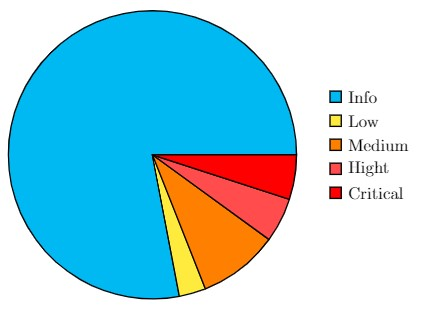
\includegraphics[width=0.6\textwidth]{images/graphiques/total.jpg}
    \caption{Vulnérabilité sur l'ensemble des machines}
    \label{fig:total}
\end{figure}

















\subsubsection{\textsc{Sovkipou.ptlab.be}}\label{app:vulns1}
Comme nous pouvons observer sur la figure \ref{fig:vuln1}, nous avons des vulnérabilités de moyenne et haute importance.
\begin{figure}[H]
    \centering
    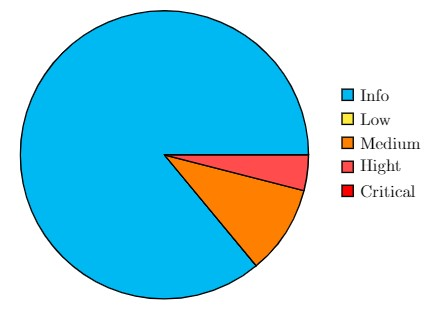
\includegraphics[width=0.6\textwidth]{images/graphiques/3.jpg}
    \caption{Vulnérabilité sur \textsc{Sovkipou.ptlab.be}}
    \label{fig:vuln1}
\end{figure}

\begin{itemize}
    \item Haute
    \begin{itemize}
        \item CVE-2016-2183 :\\
        Le chiffrement utilisé (3DES-CBC) dans le SSL n'est pas assez complexe et est susceptible d'être vulnérable à une attaque de type "Sweet32". Les ports TCP 3389/msrdp, 636/ldap, 3269/ldap sont concernés.
        \item CVE-1999-0517 :\\
        Le serveur SNMP répond aux requêtes publiques. Un attaquant peut extraire des informations utiles pour son attaque. Le port TCP 161/snmp est concerné.
    \end{itemize}
    \item Moyenne
    \begin{itemize}
        \item Certificat auto-signé :\\
        N'a pas de grande importance en interne.
        \item CVE-1999-0532 :\\
        Le serveur de noms de domaines permet d'effectuer des transferts de zones DNS. Cela peut permettre à un attaquant de facilement découvrir une liste de cibles potentielles. Le port 53/DNS est concerné.
    \end{itemize}
\end{itemize}












\subsubsection{\textsc{Soporifik.ptlab.be}}\label{app:vulns2}
Comme nous pouvons observer sur la figure \ref{fig:vuln2}, nous avons des vulnérabilités de moyenne, haute importance et des vulnérabilités critiques.
\begin{figure}[H]
    \centering
    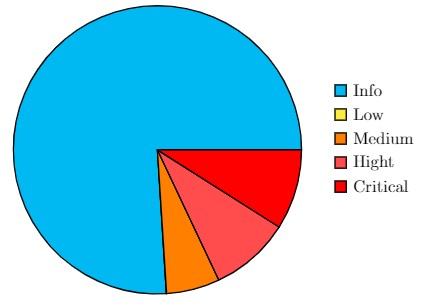
\includegraphics[width=0.6\textwidth]{images/graphiques/4.jpg}
    \caption{Vulnérabilité sur \textsc{Soporifik.ptlab.be}}
    \label{fig:vuln2}
\end{figure}

\begin{itemize}
    \item Critique
    \begin{itemize}
        \item MS06-040 :\\
        L'hôte distant est vulnérable à un dépassement de mémoire tampon dans le service 'Server' qui peut permettre à un attaquant d'exécuter du code arbitraire sur l'hôte distant avec les privilèges 'SYSTEM'.
        \item MS09-001 :\\
        L'hôte distant est affecté par une vulnérabilité de corruption de mémoire dans SMB qui peut permettre à un attaquant d'exécuter du code arbitraire ou d'effectuer un déni de service contre l'hôte distant.
        \item MS08-067 :\\
        L'hôte Windows distant est affecté par une vulnérabilité d'exécution de code à distance dans le service « Server » en raison d'une mauvaise gestion des requêtes RPC. Un attaquant distant non authentifié peut exploiter cela, via une requête RPC spécialement conçue, pour exécuter du code arbitraire avec les privilèges 'System'.
    \end{itemize}
    \item Haute
    \begin{itemize}
        \item MS17-010 (EternalBlue) :\\
        Plusieurs vulnérabilités d'exécution de code à distance existent dans Microsoft Server Message Block 1.0 (SMBv1) en raison d'une mauvaise gestion de certaines demandes. Un attaquant distant non authentifié peut exploiter ces vulnérabilités, via un paquet spécialement conçu, pour exécuter du code arbitraire. Une vulnérabilité de divulgation d'informations existe dans Microsoft Server Message Block 1.0 (SMBv1) en raison d'une mauvaise gestion de certaines demandes. Un attaquant distant non authentifié peut exploiter cela, via un paquet spécialement conçu, pour divulguer des informations sensibles. 
        \item MS06-035 :\\
        L'hôte distant est vulnérable au débordement de la heap dans le service 'Server' qui peut permettre à un attaquant d'exécuter du code arbitraire sur l'hôte distant avec les privilèges 'SYSTEM'. En plus de cela, l'hôte distant est également affecté par une vulnérabilité de divulgation d'informations dans SMB qui peut permettre à un attaquant d'obtenir des parties de la mémoire de l'hôte distant. 
        \item CVE-2002-1117 :\\
        L'hôte distant exécute Microsoft Windows. Il est possible de s'y connecter en utilisant une session NULL (c'est-à-dire sans login ni mot de passe). Selon la configuration, il est possible qu'un attaquant distant non authentifié exploite ce problème pour obtenir des informations sur l'hôte distant. 
    \end{itemize}
    \item Moyenne
    \begin{itemize}
        \item CVE-2021-36942 :\\
        Le remote host est affecté par une vulnérabilité d'élévation des privilèges de réflexion NTLM connue sous le nom de « PetitPotam ». Un attaquant distant non authentifié peut exploiter cela, en envoyant une requête EFSRPC spécialement conçue, pour forcer l'hôte affecté à se connecter à un serveur malveillant. Un attaquant peut alors utiliser un relais NTLM pour usurper l'identité de l'hôte cible et s'authentifier auprès des services distants. Un scénario d'attaque, décrit dans l'article KB5005413, utilise cet exploit pour lancer une session NTLM en tant que compte d'ordinateur d'un contrôleur de domaine. Cette session est ensuite relayée vers un hôte des services de certificats Active Directory (AD CS) pour obtenir un certificat. Ce certificat pourrait ensuite être utilisé pour se déplacer latéralement dans l'environnement du domaine.
        \item Signature SMB non requise :\\
        La signature n'est pas requise sur le serveur SMB distant. Un attaquant distant non authentifié peut exploiter cela pour mener des attaques de type man-in-the-middle contre le serveur SMB.
    \end{itemize}
\end{itemize}
















\subsubsection{\textsc{Simiabraz.ptlab.be}}\label{app:vulns3}
Comme nous pouvons observer sur la figure \ref{fig:vuln3}, nous avons une vulnérabilité moyenne.
\begin{figure}[H]
    \centering
    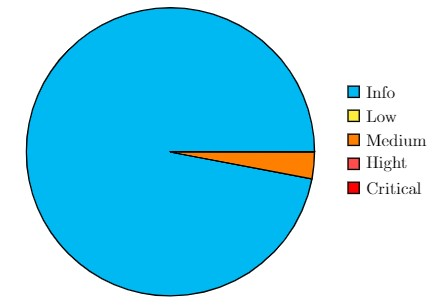
\includegraphics[width=0.6\textwidth]{images/graphiques/5.jpg}
    \caption{Vulnérabilité sur \textsc{Simiabraz.ptlab.be}}
    \label{fig:vuln3}
\end{figure}

Il s'agit de la vulnérabilité aussi présente sur \textsc{Soporifik.ptlab.be} : "Signature SMB non requise". Un attaquant distant non authentifié peut exploiter cela pour mener des attaques de type man-in-the-middle contre le serveur SMB.















\subsubsection{\textsc{Snubbull.megacorpone.be}}\label{app:vulns4}
Comme nous pouvons observer sur la figure \ref{fig:vuln4}, nous avons une vulnérabilité de basse, et moyenne importance.
\begin{figure}[H]
    \centering
    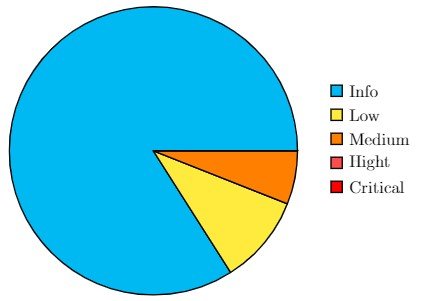
\includegraphics[width=0.6\textwidth]{images/graphiques/6.jpg}
    \caption{Vulnérabilité sur \textsc{Snubbull.megacorpone.be}}
    \label{fig:vuln4}
\end{figure}

\begin{itemize}
    \item Moyenne
    \begin{itemize}
        \item mDNS Detection :\\
        Le service distant comprend le protocole Bonjour (également connu sous le nom de ZeroConf ou mDNS), qui permet à quiconque de découvrir des informations de l'hôte distant telles que son type de système d'exploitation et sa version exacte, son nom d'hôte et la liste des services qu'il exécute.
        \item SSH Weak Algorithms Supported :\\
        Le serveur SSH distant est configuré pour utiliser le chiffrement de flux Arcfour ou aucun chiffrement. La RFC 4253 déconseille l'utilisation d'Arcfour en raison d'un problème avec des clés faibles. 
    \end{itemize}
    \item Faible
    \begin{itemize}
        \item SSH Server CBC Mode Ciphers Enabled :\\
        Le serveur SSH est configuré pour prendre en charge le chiffrement Cipher Block Chaining (CBC). Cela peut permettre à un attaquant de récupérer le message en clair à partir du texte chiffré.
        \item SSH Weak Key Exchange Algorithms Enabled : \\
        Le serveur SSH distant est configuré pour autoriser les algorithmes d'échange de clés qui sont considérés comme faibles. Ceci est basé sur le document préliminaire de l'IETF, Mises à jour et recommandations de la méthode d'échange de clés (KEX) pour Secure Shell (SSH) draft-ietf-curdle-ssh-kex-sha2-20. La section 4 énumère des conseils sur les algorithmes d'échange de clés qui NE DEVRAIENT PAS et NE DOIVENT PAS être activés.
        \item SSH Weak MAC Algorithms Enabled :\\
        Le serveur SSH distant est configuré pour autoriser les algorithmes MAC MD5 ou 96 bits, tous deux considérés comme faibles.
    \end{itemize}
\end{itemize}













\subsubsection{\textsc{Stalgamin.megacorpone.be}}\label{app:vulns5}
Comme nous pouvons observer sur la figure \ref{fig:vuln5}, nous avons une vulnérabilité moyenne et critique.
\begin{figure}[H]
    \centering
    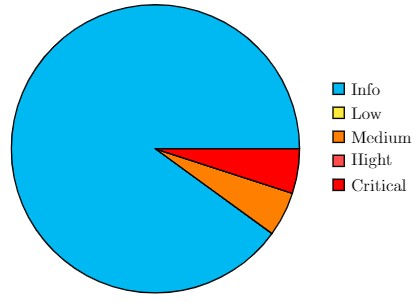
\includegraphics[width=0.6\textwidth]{images/graphiques/7.jpg}
    \caption{Vulnérabilité sur \textsc{Stalgamin.megacorpone.be}}
    \label{fig:vuln5}
\end{figure}

\begin{itemize}
    \item Critique 
    \begin{itemize}
        \item NFS Exported Share Information Disclosure (1999-0170, 1999-0554, 1999-0211) :\\
        Au moins un des partages NFS exportés par le serveur distant peut être monté par l'hôte de l'analyse. Un attaquant peut exploiter cela pour lire (et éventuellement écrire) des fichiers sur un hôte distant.
        \item CVE-2021-23017 :\\
        Selon son en-tête de réponse du serveur, la version installée de nginx est la 0.6.18 avant la 1.20.1. Il est donc affecté par une vulnérabilité d'exécution de code à distance. Un problème de sécurité dans le résolveur nginx a été identifié, ce qui pourrait permettre à un attaquant distant non authentifié de provoquer l'écrasement de la mémoire d'un octet en utilisant une réponse DNS spécialement conçue, entraînant un plantage du processus de travail ou, potentiellement, l'exécution de code arbitraire.
    \end{itemize}
    \item Moyenne
    \begin{itemize}
        \item Certificat auto-signé :\\
        N'importe qui pourrait établir une attaque de l'homme du milieu contre l'hôte distant.
        \item TLS Version 1.0 Protocol Detection :\\
        TLS 1.0 présente un certain nombre de défauts de conception cryptographique. Les serveurs qui ne sont pas activés pour TLS 1.2 et versions ultérieures ne fonctionneront plus correctement avec les principaux navigateurs Web et les principaux fournisseurs.
    \end{itemize}
\end{itemize}

\subsection{Web Application Tests}
\subsubsection{\textsc{Snubbull.megacorpone.be}}\label{app:vulns6}
Le scan WEB de Nessus a repéré 3 autres vulnérabilités moyennes et 2 basses.
\begin{itemize}
    \item Moyenne
    \begin{itemize}
        \item Browsable Web Directories :\\
        Il est possible d'identifier des dossiers car l'indexation du site est activée.
        \item Web Application Potentially Vulnerable to Clickjacking :\\
        Aucune protection contre le XSS n'est mise en place dans les headers HTTP.
        \item WordPress User Enumeration :\\
        La version de WordPress hébergée sur le serveur Web distant est affectée par une vulnérabilité d'énumération des utilisateurs. Un attaquant distant non authentifié peut exploiter cela pour connaître les noms d'utilisateurs WordPress valides. Ces informations pourraient être utilisées pour lancer d'autres attaques. 
    \end{itemize}
    \item Basse
    \begin{itemize}
        \item Web Server Transmits Cleartext Credentials :\\
        Il est conseillé de mettre les sites en HTTPS pour éviter les attaques de type man in the middle sur des pages où des données sensibles peuvent transiter, comme c'est le cas de /wordpress/wp-login.php.
        \item Web Server Allows Password Auto-Completion :
        Bien que cela ne représente pas un risque pour ce serveur Web en soi, cela signifie que les utilisateurs qui utilisent les formulaires concernés peuvent avoir leurs informations d'identification enregistrées dans leurs navigateurs, ce qui pourrait entraîner une perte de confidentialité si l'un d'entre eux utilise un hôte compromis ou si leur machine est compromise à un moment donné.
    \end{itemize}
\end{itemize}







\subsubsection{\textsc{Stalgamin.megacorpone.be}}\label{app:vulns7}

\begin{itemize}
    \item Moyenne
    \begin{itemize}
        \item Web Application Potentially Vulnerable to Clickjacking :\\
        Aucune protection contre le XSS n'est mise en place dans les headers HTTP.
    \end{itemize}
\end{itemize}






\newpage 
\addcontentsline{toc}{section}{Table des figures} \listoffigures
\newpage 
\addcontentsline{toc}{section}{Références}

\begin{thebibliography}{9}
\bibitem{1} Consulté le 13/12/2021,\\ {\small \url{https://moz.com/learn/seo/robotstxt}}
\bibitem{2} Consulté le 15/12/2021,\\ {\small \url{https://tryhackme.com/room/furthernmap}}
\bibitem{3} Consulté le 15/12/2021,\\ {\small \url{https://beaglesecurity.com/blog/vulnerability/wordpress-user-enumeration.html}}
\bibitem{4} Consulté le 16/12/2021,\\ {\small \url{https://book.hacktricks.xyz/linux-unix/privilege-escalation}}
\bibitem{5} Consulté le 18/12/2021,\\ {\small \url{https://www.xmodulo.com/update-sudo-version-linux.html}}
\bibitem{6} Consulté le 21/12/2021,\\ {\small \url{https://sushant747.gitbooks.io/total-oscp-guide/content/spawning_shells.html}}
\bibitem{7} Consulté le 15/12/2021,\\ {\small \url{https://github.com/pentestmonkey/php-reverse-shell}}
\bibitem{8} Consulté le 16/12/2021,\\ {\small \url{https://medium.com/@samsepio1/android4-vulnhub-writeup-3036f352640f}}

\end{thebibliography}












































\end{document}
